% !TeX program = xelatex
% !TeX TXS-program:compile = txs:///xelatex/[--shell-escape]
%%%%%%%%%%%%%%%%%%%%%%%%%%%%%%%%%%%%%%%%%%%%%%%%%%%%%%%%%%%%%%%%%%%%%%%%
% Plantilla TFG/TFM
% Escuela Politécnica Superior de la Universidad de Alicante
% Realizado por: Jose Manuel Requena Plens
% Contacto: info@jmrplens.com / Telegram:@jmrplens
%%%%%%%%%%%%%%%%%%%%%%%%%%%%%%%%%%%%%%%%%%%%%%%%%%%%%%%%%%%%%%%%%%%%%%%%

% Elige si deseas optimizar la ejecución del proyecto almacenando las figuras generadas con TikZ y PGF en una carpeta (archivos/figuras-procesadas).
% 1 - Si, 2 - No
\def\OptimizaTikZ{1}

% Archivo .TEX que incluye todas las configuraciones del documento y los paquetes. Añade todo aquello que necesites utilizar en el documento en este archivo.
% En él se encuentra la configuración de los márgenes, establecidos según las directrices de estilo de la EPS.
%%%%%%%%%%%%%%%%%%%%%%%%%%%%%%%%%%%%%%%%%%%%%%%%%%%%%%%%%%%%%%%%%%%%%%%%
% Plantilla TFG/TFM
% Escuela Politécnica Superior de la Universidad de Alicante
% Realizado por: Jose Manuel Requena Plens
% Contacto: info@jmrplens.com / Telegram:@jmrplens
%%%%%%%%%%%%%%%%%%%%%%%%%%%%%%%%%%%%%%%%%%%%%%%%%%%%%%%%%%%%%%%%%%%%%%%%

%%%%%%%%%%%%%%%%%%%%%%%%
% FORMATO DEL DOCUMENTO
%%%%%%%%%%%%%%%%%%%%%%%%
% scrbook es la clase de documento
% Si se desea que no haya página en blanco entre capítulos añadir "openany" en los parámetros de la clase. Sino siempre los capítulos empezarán en página impar.
\documentclass[a4paper,11pt,titlepage]{scrbook}
\KOMAoption{toc}{bib,chapterentryfill} % Opciones del índice
\usepackage{scrhack} % Previene algunos errores
% Paquete de formato para scrbook. Con marcas, linea-separador superior e inferior
\usepackage[automark,headsepline,footsepline]{scrlayer-scrpage}
\clearpairofpagestyles		% Borra los estilos por defecto
%%
% Formato y contenido de la información de cabecera y pie de página
%%
% Información de capítulo en cabecera e interno
\ihead{{\color{gray30}\scshape\small\headmark}}	
% Número de página en cabecera y externo
\ohead{\normalfont\pagemark} 
% Número de página en pie de página y externo. Sólo en páginas sin cabecera
\ofoot[\normalfont\pagemark]{}
%% 		
% Edición del contenido de las distintas partes de la cabecera
%%
\renewcommand{\chaptermark}[1]{\markboth{#1}{}} % Capítulo (Solo texto)
\renewcommand{\sectionmark}[1]{\markright{\thesection. #1}} % Sección (Número y texto)
\setkomafont{pagenumber}{} % Número de página (Sin nada añadido)

% Añade al índice y numera hasta la profundidad 4.
% 1:section,2:subsection,3:subsubsection,4:paragraph
\setcounter{tocdepth}{4}
\setcounter{secnumdepth}{4}
% Muestra una regla para comprobar el formato de las páginas
%\usepackage[type=upperleft,showframe,marklength=8mm]{fgruler}
% MÁRGENES DE LAS PÁGINAS
\usepackage[
  inner	=	3.0cm, % Margen interior
  outer	=	2.5cm, % Margen exterior
  top	=	2.5cm, % Margen superior
  bottom=	2.5cm, % Margen inferior
  includeheadfoot, % Incluye cabecera y pie de página en los márgenes
]{geometry}
% Valor de interlineado
\renewcommand{\baselinestretch}{1.0} % 1 línea de interlineado
% Para poder generar páginas horizontales
\usepackage{lscape}
% Ancho de la zona para comentarios en el margen. (modificado para todonotes)
\setlength{\marginparwidth}{1.9cm}

%%%%%%%%%%%%%%%%%%%%%%%%
% BIBLIOGRAFÍA
%%%%%%%%%%%%%%%%%%%%%%%%
\usepackage{apacite} % NORMA APA
\usepackage{natbib}
\usepackage{breakcites}

%%%%%%%%%%%%%%%%%%%%%%%%
% DOCUMENTO EN ESPAÑOL
%%%%%%%%%%%%%%%%%%%%%%%%
\usepackage[base]{babel}
\usepackage{polyglossia}
\setdefaultlanguage{spanish}

\addto\captionsspanish{%
	\renewcommand{\listtablename}{Índice de tablas} 
	\renewcommand{\tablename}{Tabla}
	\renewcommand{\lstlistingname}{Código}
	\renewcommand{\lstlistlistingname}{Índice de \lstlistingname s}
	\renewcommand{\glossaryname}{Glosario}
	\renewcommand{\acronymname}{Acrónimos}
	\renewcommand{\bibname}{Bibliografía}%
}

%%%%%%%%%%%%%%%%%%%%%%%% 
% COLORES
%%%%%%%%%%%%%%%%%%%%%%%% 
% Biblioteca de colores
\usepackage{color}
\usepackage[dvipsnames]{xcolor}
% Otros colores definidos por el usuario
\definecolor{gray97}{gray}{.97}
\definecolor{gray75}{gray}{.75}
\definecolor{gray45}{gray}{.45}
\definecolor{gray30}{gray}{.30}
\definecolor{negro}{RGB}{0,0,0}
\definecolor{blanco}{RGB}{255,255,255}
\definecolor{dkgreen}{rgb}{0,.6,0}
\definecolor{dkblue}{rgb}{0,0,.6}
\definecolor{dkyellow}{cmyk}{0,0,.8,.3}
\definecolor{gray}{rgb}{0.5,0.5,0.5}
\definecolor{mauve}{rgb}{0.58,0,0.82}
\definecolor{deepblue}{rgb}{0,0,0.5}
\definecolor{deepred}{rgb}{0.6,0,0}
\definecolor{deepgreen}{rgb}{0,0.5,0}
\definecolor{MyDarkGreen}{rgb}{0.0,0.4,0.0}
\definecolor{bluekeywords}{rgb}{0.13,0.13,1}
\definecolor{greencomments}{rgb}{0,0.5,0}
\definecolor{redstrings}{rgb}{0.9,0,0}

%%%%%%%%%%%%%%%%%%%%%%%%
% TABLAS
%%%%%%%%%%%%%%%%%%%%%%%%
% Paquetes para tablas
\usepackage{longtable,booktabs,array,multirow,multicol,tabularx,ragged2e,array}
% Nuevos tipos de columna para tabla, se pueden utilizar como por ejemplo C{3cm} en la definición de columnas de la función tabular
\newcolumntype{L}[1]{>{\raggedright\let\newline\\\arraybackslash\hspace{0pt}}m{#1}}
\newcolumntype{C}[1]{>{\centering\let\newline\\\arraybackslash\hspace{0pt}}m{#1}}
\newcolumntype{R}[1]{>{\raggedleft\let\newline\\\arraybackslash\hspace{0pt}}m{#1}}

%%%%%%%%%%%%%%%%%%%%%%%% 
% GRAFICAS y DIAGRAMAS 
%%%%%%%%%%%%%%%%%%%%%%%% 
% Paquete para todo tipo de gráficas, diagramas, modificación de imágenes, etc
\usepackage{tikz,tikzpagenodes}
\usetikzlibrary{tikzmark,calc,shapes.geometric,arrows,backgrounds,shadings,shapes.arrows,shapes.symbols,shadows,positioning,fit,automata,patterns,intersections}
\usepackage{pgfplots}
\pgfplotsset{colormap/jet}
\pgfplotsset{compat=newest} % Compatibilidad
\usepgfplotslibrary{patchplots,groupplots,fillbetween,polar}
\usepackage{pgfplotstable}
% Guardar las figuras realizadas con Tikz y Pgf en una carpeta externa
% para agilizar el procesado y tenerlas para utilizarlas en otros
% documentos
\if\OptimizaTikZ 1
\usepgfplotslibrary{external}
\tikzexternalize[prefix=archivos/figuras-procesadas/] % Ruta
\tikzset{%
    external/system call ={xelatex -enable-write18 -halt-on-error -interaction=batchmode -jobname "\image" "\texsource"},
}
\fi

% Estilos para elementos graficos
% Cajas y cajas de texto
\tikzstyle{Caja1} = [green,very thick,rounded corners,fill=white, fill opacity=0.5]
\tikzstyle{Texto1} = [fill=white,thick,shape=circle,draw=black,inner sep=2pt,font=\sffamily,text=black]
\tikzstyle{Texto2} = [fill=white,thick,shape=rectangle,draw=black,inner sep=2pt,font=\sffamily,text=black]
\tikzstyle{Texto3} = [fill=white,thick,shape=circle,draw=black,inner sep=2pt,font=\sffamily,text=black]
% Cuadros de diagrama
\tikzstyle{rectvioleta} = [rectangle, rounded corners, text centered, draw=black, fill=blue!10]
\tikzstyle{rectnaranja} = [rectangle, minimum width=2cm, minimum height=1cm, text centered, draw=black, fill=orange!10]
\tikzstyle{romborosa} = [diamond, aspect=3, minimum width=3cm, minimum height=1cm, text centered, draw=black, fill=red!10]
\tikzstyle{rectverde} = [rectangle, minimum width=2cm, minimum height=1cm, text centered, draw=black, fill=green!10]
\tikzstyle{rectamarillo} = [rectangle, rounded corners, minimum width=2cm, minimum height=1cm, text centered, draw=black, fill=yellow!10]
% Flechas
\tikzstyle{arrow} = [thick,->,>=stealth]

%%%%%%%%%%%%%%%%%%%%%%%% 
% FIGURAS, TABLAS, ETC 
%%%%%%%%%%%%%%%%%%%%%%%% 
\usepackage{subcaption} % Para poder realizar subfiguras
\usepackage{caption} % Para aumentar las opciones de diseño
% Nombres de figuras, tablas, etc, en negrita la numeración, todo con letra small
\captionsetup{labelfont={bf,small},textfont=small}
% Paquete para modificar los espacios arriba y abajo de una figura o tabla
\usepackage{setspace}
% Define el espacio tanto arriba como abajo de las figuras, tablas
\setlength{\intextsep}{5mm}
% Para ajustar tamaños de texto de toda una tabla o grafica
% Uso: {\scalefont{0.8} \begin{...} \end{...} }
\usepackage{scalefnt}
% Redefine las tablas y figuras para eliminar el '.' entre la numeración y el texto
\renewcommand*{\figureformat}{\figurename~\thefigure}
\renewcommand*{\tableformat}{\tablename~\thetable}

%%%%%%%%%%%%%%%%%%%%%%%% 
% TEXTO
%%%%%%%%%%%%%%%%%%%%%%%%
% Paquete para poder modificar las fuente de texto
\usepackage{xltxtra}
% Cualquier tamaño de texto. Uso: {\fontsize{100pt}{120pt}\selectfont tutexto}
\usepackage{anyfontsize}
% Para modificar parametros del texto.
\usepackage{setspace}
% Paquete para posicionar bloques de texto
\usepackage{textpos}
% Paquete para realizar cajas de texto. 
% Uso: \begin{mdframed}[linecolor=red!100!black] tutexto \end{mdframed}
\usepackage{framed,mdframed}
% Para subrayar. Uso: \hlc[tucolor]{tutexto}
\newcommand{\hlc}[2][yellow]{ {\sethlcolor{#1} \hl{#2}} }

%%%%%%%%%%%%%%%%%%%%%%%% 
% OTROS
%%%%%%%%%%%%%%%%%%%%%%%%
% Para hacer una pagina horizontal. Uso: \begin{landscape} xxxx \end{lanscape}
\usepackage{lscape} 
% Para incluir paginas PDF. Uso:
% \includepdf[pages={1}]{tuarchivo.pdf}
\usepackage{pdfpages}
% Para introducir url's con formato. Uso: \url{http://www.google.es}
\usepackage{url}
% Amplia muchas funciones graficas de latex
\usepackage{graphicx}
% Paquete que añade el hipervinculo en referencias dentro del documento, indice, etc
% Se define sin bordes alrededor. Uso: \ref{tulabel}
\usepackage[pdfborder={000}]{hyperref}
\usepackage{float}
\usepackage{placeins}
\usepackage{afterpage}
\usepackage{verbatim}
% Paquete para condicionales avanzados
\usepackage{xstring,xifthen}
% Paquete para realizar calculos en el código
\usepackage{calc}
% Para rotar tablas o figuras o su contenido
\usepackage{rotating} 
% Para incluir comentarios en el texto. El parámetro 'disable' oculta todas las notas.
% USO: \todo{tutexto}
\usepackage[textsize=tiny,spanish,shadow,textwidth=2cm]{todonotes}
%\reversemarginpar % Descomentar si se quiere todos los comentarios en el mismo lado
% Desactiva la exportación de los ToDo y Missingfigures como figuras
\if\OptimizaTikZ 1
\makeatletter
\renewcommand{\todo}[2][]{\tikzexternaldisable\@todo[#1]{#2}\tikzexternalenable}
\makeatother
\usepackage{letltxmacro}
\LetLtxMacro{\oldmissingfigure}{\missingfigure}
\makeatletter
\renewcommand{\missingfigure}[2][]{\tikzexternaldisable\oldmissingfigure[{#1}]{#2}\tikzexternalenable}
\makeatother
\fi

%%%%%%%%%%%%%%%%%%%%%%%% 
% GLOSARIOS
%%%%%%%%%%%%%%%%%%%%%%%%
\usepackage[acronym,nonumberlist,toc]{glossaries}
\usepackage{glossary-superragged}
\newglossarystyle{modsuper}{%
  \setglossarystyle{super}%
  \renewcommand{\glsgroupskip}{}
}
\renewcommand{\glsnamefont}[1]{\textbf{#1}}


%%%%%%%%%%%%%%%%%%%%%%%% 
% COMANDOS AÑADIDOS
%%%%%%%%%%%%%%%%%%%%%%%%
% Para mostrar la fecha actual (mes año) con \Hoy
\newcommand{\MES}{%
  \ifcase\month% 0
    \or Enero% 1
    \or Febrero% 2
    \or Marzo% 3
    \or Abril% 4
    \or Mayo% 5
    \or Junio% 6
    \or Julio% 7
    \or Agosto% 8
    \or Septiembre% 9
    \or Octubre% 10
    \or Noviembre% 11
    \or Diciembre% 12
  \fi}
\newcommand{\ANYO}{\number\year}
\newcommand{\Hoy}{\MES\ \ANYO}

%%%%%%%%%%%%%%%%%%%%%%%% 
% MATEMÁTICAS
%%%%%%%%%%%%%%%%%%%%%%%%
\usepackage{mathtools,amsthm,amsfonts,amssymb,bm,mathrsfs,nicefrac,upgreek,bigints} 
% Comando para añadir información de variables a las ecuaciones
% Uso: \begin{condiciones}[donde:] ....... \end{condiciones}
\newenvironment{condiciones}[1][2]
  {%
   #1\tabularx{\textwidth-\widthof{#1}}[t]{
     >{$}l<{$} @{}>{${}}c<{{}$}@{} >{\raggedright\arraybackslash}X
   }%
  }
  {\endtabularx\\[\belowdisplayskip]}

%%%%%
% PARÁMETROS DE FORMATO DE CODIGOS
%%%%%
% Puedes editar los formatos para ajustarlos a tu gusto
%%%%%%%%%%%%%%%%%%%%%%%%%%%%%%%%%%%%%%%%%%%%%%%%%%%%%%%%%%%%%%%%%%%%%%%%
% Plantilla TFG/TFM
% Escuela Politécnica Superior de la Universidad de Alicante
% Realizado por: Jose Manuel Requena Plens
% Contacto: info@jmrplens.com / Telegram:@jmrplens
%%%%%%%%%%%%%%%%%%%%%%%%%%%%%%%%%%%%%%%%%%%%%%%%%%%%%%%%%%%%%%%%%%%%%%%%


%%%%%%%%%%%%%%%%%%%%%%%% 
% CÓDIGO. CONFIGURACIÓN. En el siguiente bloque están los estilos.
%%%%%%%%%%%%%%%%%%%%%%%%
% Paquete para mostrar código de matlab. En caja y lineas numeradas
\usepackage[framed,numbered]{matlab-prettifier}
% Paquete mostrar código de programación de distintos lenguajes
\usepackage{listings}
\lstset{ inputencoding=utf8,
extendedchars=true,
frame=single, % Caja donde se ubica el código
backgroundcolor=\color{gray97}, % Color del fondo de la caja
rulesepcolor=\color{black},
boxpos=c,
abovecaptionskip=-4pt,
aboveskip=12pt,
belowskip=0pt,
lineskip=0pt,
framerule=0pt,
framextopmargin=4pt,
framexbottommargin=4pt,
framexleftmargin=11pt,
framexrightmargin=0pt,
linewidth=\linewidth,
xleftmargin=\parindent,
framesep=0pt,
rulesep=.4pt,
stringstyle=\ttfamily,
showstringspaces = false,
showspaces = false,
showtabs = false,
columns=fullflexible,
basicstyle=\small\ttfamily,
commentstyle=\color{gray45},
keywordstyle=\bfseries,
tabsize=4,
numbers=left,
numbersep=1pt,
numberstyle=\tiny\ttfamily\color{gray75},
numberfirstline = false,
breaklines=true,
postbreak=\mbox{\textcolor{red}{$\hookrightarrow$}\space}, % Flecha al saltar de linea
prebreak=\mbox{\textcolor{red}{$\hookleftarrow$}\space}, % Flecha al saltar de linea
literate=
  {á}{{\'a}}1 {é}{{\'e}}1 {í}{{\'i}}1 {ó}{{\'o}}1 {ú}{{\'u}}1
  {Á}{{\'A}}1 {É}{{\'E}}1 {Í}{{\'I}}1 {Ó}{{\'O}}1 {Ú}{{\'U}}1
  {à}{{\`a}}1 {è}{{\`e}}1 {ì}{{\`i}}1 {ò}{{\`o}}1 {ù}{{\`u}}1
  {À}{{\`A}}1 {È}{{\'E}}1 {Ì}{{\`I}}1 {Ò}{{\`O}}1 {Ù}{{\`U}}1
  {ä}{{\"a}}1 {ë}{{\"e}}1 {ï}{{\"i}}1 {ö}{{\"o}}1 {ü}{{\"u}}1
  {Ä}{{\"A}}1 {Ë}{{\"E}}1 {Ï}{{\"I}}1 {Ö}{{\"O}}1 {Ü}{{\"U}}1
  {â}{{\^a}}1 {ê}{{\^e}}1 {î}{{\^i}}1 {ô}{{\^o}}1 {û}{{\^u}}1
  {Â}{{\^A}}1 {Ê}{{\^E}}1 {Î}{{\^I}}1 {Ô}{{\^O}}1 {Û}{{\^U}}1
  {œ}{{\oe}}1 {Œ}{{\OE}}1 {æ}{{\ae}}1 {Æ}{{\AE}}1 {ß}{{\ss}}1
  {ű}{{\H{u}}}1 {Ű}{{\H{U}}}1 {ő}{{\H{o}}}1 {Ő}{{\H{O}}}1
  {ç}{{\c c}}1 {Ç}{{\c C}}1 {ø}{{\o}}1 {å}{{\r a}}1 {Å}{{\r A}}1
  {€}{{\euro}}1 {£}{{\pounds}}1 {«}{{\guillemotleft}}1
  {»}{{\guillemotright}}1 {ñ}{{\~n}}1 {Ñ}{{\~N}}1 {¿}{{?`}}1,
  }

% Intenta no dividir los códigos en diferentes paginas si es posible
\lstnewenvironment{listing}[1][]
   {\lstset{#1}\pagebreak[0]}{\pagebreak[0]}

% Formato de títulos de los códigos
\DeclareCaptionFont{white}{\color{white}}
\DeclareCaptionFormat{listing}{\colorbox{gray}{\parbox{\textwidth - 2\fboxsep}{#1#2#3}}}
\captionsetup[lstlisting]{format=listing,labelfont=white,textfont=white,font= scriptsize}


%%%%%%%%%%%%%%%%%%%%%%%% 
% CÓDIGO. ESTILOS. Ajústalos a tu gusto
%%%%%%%%%%%%%%%%%%%%%%%%
\lstdefinestyle{Consola}
	{
	basicstyle=\scriptsize\bf\ttfamily,
	}
   
\lstdefinestyle{C}
	{
	basicstyle=\scriptsize,
	language=C,
	}
\lstdefinestyle{C-color}
	{
  	breaklines=true,
  	language=C,
  	basicstyle=\scriptsize,
  	keywordstyle=\bfseries\color{green!40!black},
  	commentstyle=\itshape\color{purple!40!black},
  	identifierstyle=\color{blue},
  	stringstyle=\color{orange},
    }
\lstdefinestyle{CSharp}
	{
	basicstyle=\scriptsize
	language=[Sharp]C,
	escapeinside={(*@}{@*)},
	keywordstyle=\bfseries,
	}
\lstdefinestyle{CSharp-color}
	{
	basicstyle=\scriptsize
	language=[Sharp]C,
	escapeinside={(*@}{@*)},
	commentstyle=\color{greencomments},
	keywordstyle=\color{bluekeywords}\bfseries,
	stringstyle=\color{redstrings},
	}
\lstdefinestyle{C++}
	{
	basicstyle=\scriptsize,
	language=C++,
 	}
 	
\lstdefinestyle{C++-color}
	{
  	breaklines=true,
  	language=C++,
  	basicstyle=\scriptsize,
  	keywordstyle=\bfseries\color{green!40!black},
  	commentstyle=\itshape\color{purple!40!black},
  	identifierstyle=\color{blue},
  	stringstyle=\color{orange},
    }
    
\lstdefinestyle{PHP}
	{
	basicstyle=\scriptsize,
	language=PHP,
	}
	
\lstdefinestyle{PHP-color}
	{
	basicstyle=\scriptsize,
	language=PHP,
	keywordstyle    = \color{dkblue},
  	stringstyle     = \color{red},
  	identifierstyle = \color{dkgreen},
  	commentstyle    = \color{gray},
  	emph            =[1]{php},
  	emphstyle       =[1]\color{black},
  	emph            =[2]{if,and,or,else},
  	emphstyle       =[2]\color{dkyellow}
  }
  
\lstdefinestyle{Matlab}
	{
	basicstyle=\scriptsize,
	language=Matlab,
	numberstyle=\tiny\ttfamily\color{gray75},
	}
	
\lstdefinestyle{Matlab-color}
	{
	style = Matlab-editor,
	basicstyle=\scriptsize,
	numberstyle=\tiny\ttfamily\color{gray75},
	}
	
\lstdefinestyle{Latex}
	{
	language=[LaTeX]{Tex},
    basicstyle=\scriptsize,
    literate={\$}{{{\bfseries\$}}}1,
    alsoletter={\\,*,\&},
    emph =[1]{\\begin,\\end,\\caption,\\label,\\centering,\\FloatBarrier,
              \\lstinputlisting,\\scalefont,\\addplot,\\input,
              \\legend,\\item,\\subitem,\\includegraphics,\\textwidth,
              \\section,\\subsection,\\subsubsection,\\paragraph,
              \\cite,\\citet,\\citep,\\gls,\\bibliographystyle,\\url,
              \\citet*,\\citep*,\\todo,\\missingfigure,\\footnote},
  	emphstyle =[1]\bfseries,
  	emph = [2]{equation,subequations,eqnarray,figure,subfigure,
  			   condiciones,flalign,tikzpicture,axis,lstlisting,
  			   itemize,description
  			   },
  	emphstyle =[2]\bfseries,
    numbers=none,
	}
	
\lstdefinestyle{Latex-color}
	{
	language=[LaTeX]{Tex},
    basicstyle=\scriptsize,
    commentstyle=\color{dkgreen},
    identifierstyle=\color{black},
    literate={\$}{{{\bfseries\color{Dandelion}\$}}}1, % Colorea el simbolo dollar
    alsoletter={\\,*,\&},
    emph =[1]{\\begin,\\end,\\caption,\\label,\\centering,\\FloatBarrier,
              \\lstinputlisting,\\scalefont,\\addplot,\\input,
              \\legend,\\item,\\subitem,\\includegraphics,\\textwidth,
              \\section,\\subsection,\\subsubsection,\\paragraph,
              \\cite,\\citet,\\citep,\\gls,\\bibliographystyle,\\url,
              \\citet*,\\citep*,\\todo,\\missingfigure,\\footnote},
  	emphstyle =[1]\bfseries\color{RoyalBlue},
  	emph = [2]{equation,subequations,eqnarray,figure,subfigure,
  			   condiciones,flalign,tikzpicture,axis,lstlisting,
  			   itemize,description
  			   },
  	emphstyle =[2]\bfseries,
    numbers=none,
	}
\lstdefinestyle{Java}
{
	basicstyle=\scriptsize,
	language=Java,
}

\lstdefinestyle{Java-color}
{
	basicstyle=\scriptsize,
	language=Java,
  	keywordstyle=\color{blue},
  	commentstyle=\color{dkgreen},
  	stringstyle=\color{mauve},
}
\lstdefinestyle{Python}
{
	language=Python,
	basicstyle=\scriptsize,
	otherkeywords={self},  
	keywordstyle=\bfseries,     
	emphstyle=\bfseries,    
	emph={MyClass,__init__},         
}

\lstdefinestyle{Python-color}
{
	language=Python,
	basicstyle=\scriptsize,
	otherkeywords={self},          
	keywordstyle=\bfseries\color{deepblue},
	emph={MyClass,__init__},         
	emphstyle=\bfseries\color{deepred},    
	stringstyle=\color{deepgreen},
}
\lstdefinestyle{R}
{
	language=R,                     
  	basicstyle=\scriptsize,
  	keywordstyle=\bfseries, 
}
\lstdefinestyle{R-color}
{
	language=R,                     
  	basicstyle=\scriptsize,
  	keywordstyle=\bfseries\color{RoyalBlue}, 
  	commentstyle=\color{YellowGreen},
  	stringstyle=\color{ForestGreen}  
}


%%%%%
% DEFINICION DE CONCEPTOS
%%%%
% Uso ejemplo: \begin{ejemplo} tucontenido \end{ejemplo} 
\newtheorem{teorema}{Teorema}[chapter]
\newtheorem{ejemplo}{Ejemplo}[chapter]
\newtheorem{definicion}{Definición}[chapter]



%%%%%%%%%%%%%%%%%%%%%%%%%%%%%%%%%%%%%%%%%%%%%%%%%%%%%%%%%%%%%%%%%%%%%%
% INFORMACIÓN DEL TFG
% Comentar lo que NO se desee añadir y sustituir con la información correcta.
%%%%%%%%%%%%%%%%%%%%%%%%%%%%%%%%%%%%%%%%%%%%%%%%%%%%%%%%%%%%%%%%%%%%%%
% Título y subtítulo
\newcommand{\titulo}{Título del Trabajo Fin de Grado/Máster}
\newcommand{\subtitulo}{Subtítulo del proyecto}
% Datos del autor
\newcommand{\miNombre}{Nombre Apellido1 Apellido2 (alumno)}
% Determinar género para etiquetas Autore/Autora/Autor (nb o en blanco,f,m)
\newcommand{\miGenero}{m}
\newcommand{\miEmail}{nombre@alu.ua.es}
% Datos del tutor/es
% Si no hay tutorB, comentar tutorB y dptoB para que la etiqueta sea Tutor:
\newcommand{\miTutor}{Nombre Apellido1 Apellido2 (tutor1)}
\newcommand{\miTutorB}{Nombre Apellido1 Apellido2 (tutor2)}
\newcommand{\departamentoTutor}{Departamento del tutor}
\newcommand{\departamentoTutorB}{Departamento del cotutor}
% Datos de la facultad y universidad
\newcommand{\miFacultad}{Escuela Politécnica Superior}
\newcommand{\miFacultadCorto}{EPS UA}
\newcommand{\miUniversidad}{\protect{Universidad de Alicante}}
\newcommand{\miUbicacion}{Alicante}

%%%%%%%%%%%%%%%%%%%%%%%%%%%%%%%%%%%%%%%%%%%%%%%%%%%%%%%%%%%%%%%%%%%%%%
% INDICA TU TITULACIÓN
% ID	GRADO -------------------------------------------------
% 1		Ingeniería en Imagen y Sonido en Telecomunicación
% 2		Ingeniería Civil
% 3		Ingeniería Química
% 4		Ingeniería Informática
% 5		Ingeniería Multimedia
% 6		Arquitectura Técnica
% 7		Arquitectura
% 8		Robótica
% %		%%%%%%%%%%%%
% ID	MÁSTER ------------------------------------------------
% A		Telecomunicación
% B		Caminos, Canales y Puertos
% C		Gestión en la Edificación
% D		Desarrollo Web
% E		Materiales, Agua, Terreno
% F		Informática
% G 	Automática y Robótica
% H		Prevención de riesgos laborales
% I		Gestión Sostenible Agua
% J		Desarrollo Aplicaciones Móviles
% K		Ingeniería Química
% L		Ciberseguridad
%%%%%%%%%%%%%%%%%%%%%%%%%%%%%%%%%%%%%%%%%%%%%%%%%%%%%%%%%%%%%%%%%%%%%%%%%
%!!!!!!!!!!!!!!!!!!!!!!!!!!!!!!!!!!!!!!!!!!!!!!!!!!!!!!!!!!!!!!!!!!!!!%%%
																		%
\def\IDtitulo{1} % INTRODUCE LA ID DE TU TITULACIÓN						%
																		%
%!!!!!!!!!!!!!!!!!!!!!!!!!!!!!!!!!!!!!!!!!!!!!!!!!!!!!!!!!!!!!!!!!!!!!%%%
%%%%%%%%%%%%%%%%%%%%%%%%%%%%%%%%%%%%%%%%%%%%%%%%%%%%%%%%%%%%%%%%%%%%%%%%%

% Configuración automática según el identificador elegido
%%%%%%%%%%%%%%%%%%%%%%%%%%%%%%%%%%%%%%%%%%%%%%%%%%%%%%%%%%%%%%%%%%%%%%%%
% Plantilla TFG/TFM
% Escuela Politécnica Superior de la Universidad de Alicante
% Realizado por: Jose Manuel Requena Plens
% Contacto: info@jmrplens.com / Telegram:@jmrplens
%%%%%%%%%%%%%%%%%%%%%%%%%%%%%%%%%%%%%%%%%%%%%%%%%%%%%%%%%%%%%%%%%%%%%%%%

%%%%%%%%%%%%%%%%%%%%%%%% 
% COLORES DE GRADOS.
% Si el color de la titulación ha cambiado, modifícalo en las lineas siguientes.
%%%%%%%%%%%%%%%%%%%%%%%%
% Grados
\definecolor{teleco}{RGB}{32,2,116}			% Teleco
\definecolor{civil}{RGB}{201,56,140}			% Civil
\definecolor{quimica}{RGB}{41,199,255}		% Química
\definecolor{informatica}{RGB}{0,128,255}	% Informatica
\definecolor{multimedia}{RGB}{239,206,53}	% Multimedia
\definecolor{arquitecnica}{RGB}{0,179,148}	% Arquitectura técnica
\definecolor{arquitectura}{RGB}{181,0,0}		% Arquitectura
\definecolor{robotica}{RGB}{255,255,128}		% Robótica
% Másteres
\definecolor{masterteleco}{RGB}{32,2,116}	% Teleco
\definecolor{caminos}{RGB}{201,56,140}		% Caminos, Canales y Puertos
\definecolor{gestedif}{RGB}{50,120,50}		% Gestión Edificación
\definecolor{desweb}{RGB}{250,43,22}			% Desarrollo Web
\definecolor{mataguaterre}{RGB}{210,250,50}	% Materiales, Agua, Terreno
\definecolor{masterinfor}{RGB}{0,128,255}	% Informática
\definecolor{autorobo}{RGB}{83,145,201}		% Automática y Robótica
\definecolor{prevencion}{RGB}{0,100,0}		% Prevención Riesgos
\definecolor{gestionagua}{RGB}{7,138,197}	% Gestión Agua
\definecolor{moviles}{RGB}{121,11,21}		% Aplicaciones Móviles
\definecolor{masterquimica}{RGB}{41,199,255}	% Quimica
\definecolor{ciberseguridad}{RGB}{9,111,192}	% Ciberseguridad

% Logotipos comunes de todas las titulaciones
\newcommand{\logoFacultad}{include/logos-universidad/LogoEPSNegro}
\newcommand{\logoUniversidad}{include/logos-universidad/LogoUANegro}
\newcommand{\logoUniversidadPortada}{include/logos-universidad/LogoUABlanco}

% Colores generales
\definecolor{negro}{RGB}{0,0,0}
\definecolor{blanco}{RGB}{255,255,255}
%%%%%%%%%%%%%%%%%%%%%%%% 
% CONDICIONALES. SEGUN LA ID ELEGIDA EN EL .TEX PRINCIPAL
% Según el ID seleccionado en TFG_EPS_UA.tex se configurará el nombre de la titulación, logotipos y color.
% Si tu titulación no esta correctamente definida cambia las imágenes que se definen para tu titulación en las lineas de abajo
% Si deseas añadir mas titulaciones ve al final de este archivo
%%%%%%%%%%%%%%%%%%%%%%%%
% Grados
	\if\IDtitulo 1 % Teleco
		% Logos
		\newcommand{\logoFacultadPortada}{include/logos-universidad/LogoEPSBlanco}
		\newcommand{\logoGradoPortada}{include/logos-titulaciones/LogoTelecoBlanco}
		\newcommand{\logoGrado}{include/logos-titulaciones/LogoTelecoNegro}
		% Texto
		\newcommand{\miGrado}{Grado en Ingeniería en Sonido e Imagen en Telecomunicación}
		\newcommand{\tipotrabajo}{Trabajo Fin de Grado}
		% Color
		\newcommand{\colorgrado}{teleco}
		\newcommand{\colortexto}{blanco}
	\else \if\IDtitulo 2 % Civil
		\newcommand{\logoFacultadPortada}{include/logos-universidad/LogoEPSBlanco}
		\newcommand{\logoGradoPortada}{include/logos-titulaciones/LogoCivilBlanco}
		\newcommand{\logoGrado}{include/logos-titulaciones/LogoCivilNegro}
		% Texto
		\newcommand{\miGrado}{Grado en Ingeniería Civil}
		\newcommand{\tipotrabajo}{Trabajo Fin de Grado}
		% Color
		\newcommand{\colorgrado}{civil}
		\newcommand{\colortexto}{blanco}
	\else \if\IDtitulo 3 % Quimica
		% Logos
		\newcommand{\logoFacultadPortada}{include/logos-universidad/LogoEPSNegro}
		\newcommand{\logoGradoPortada}{include/logos-titulaciones/LogoQuimicaNegro}
		\newcommand{\logoGrado}{include/logos-titulaciones/LogoQuimicaNegro}
		% Texto
		\newcommand{\miGrado}{Grado en Ingeniería Química}
		\newcommand{\tipotrabajo}{Trabajo Fin de Grado}
		% Color
		\newcommand{\colorgrado}{quimica}
		\newcommand{\colortexto}{negro}
	\else \if\IDtitulo 4 % Informatica
		% Logos
		\newcommand{\logoFacultadPortada}{include/logos-universidad/LogoEPSBlanco}
		\newcommand{\logoGradoPortada}{include/logos-titulaciones/LogoInformaticaBlanco}
		\newcommand{\logoGrado}{include/logos-titulaciones/LogoInformaticaNegro}
		% Texto
		\newcommand{\miGrado}{Grado en Ingeniería Informática}
		\newcommand{\tipotrabajo}{Trabajo Fin de Grado}
		% Color
		\newcommand{\colorgrado}{informatica}
		\newcommand{\colortexto}{blanco}
	\else \if\IDtitulo 5 % Multimedia
		% Logos
		\newcommand{\logoFacultadPortada}{include/logos-universidad/LogoEPSNegro}
		\newcommand{\logoGradoPortada}{include/logos-titulaciones/LogoMultimediaNegro}
		\newcommand{\logoGrado}{include/logos-titulaciones/LogoMultimediaNegro}
		% Texto
		\newcommand{\miGrado}{Grado en Ingeniería Multimedia}
		\newcommand{\tipotrabajo}{Trabajo Fin de Grado}
		% Color
		\newcommand{\colorgrado}{multimedia}
		\newcommand{\colortexto}{negro}
	\else \if\IDtitulo 6 % Arquitectura Tecnica
		% Logos
		\newcommand{\logoFacultadPortada}{include/logos-universidad/LogoEPSBlanco}
		\newcommand{\logoGradoPortada}{include/logos-titulaciones/LogoArqTecnicaBlanco}
		\newcommand{\logoGrado}{include/logos-titulaciones/LogoArqTecnicaNegro}
		% Texto
		\newcommand{\miGrado}{Grado en Arquitectura Técnica}
		\newcommand{\tipotrabajo}{Trabajo Fin de Grado}
		% Color
		\newcommand{\colorgrado}{arquitecnica}
		\newcommand{\colortexto}{blanco}
	\else \if\IDtitulo 7 % Arquitectura
		% Logos
		\newcommand{\logoFacultadPortada}{include/logos-universidad/LogoEPSBlanco}
		\newcommand{\logoGradoPortada}{include/logos-titulaciones/LogoArquitecturaBlanco}
		\newcommand{\logoGrado}{include/logos-titulaciones/LogoArquitecturaNegro}
		% Texto
		\newcommand{\miGrado}{Grado en Arquitectura}
		\newcommand{\tipotrabajo}{Trabajo Fin de Grado}
		% Color
		\newcommand{\colorgrado}{arquitectura}
		\newcommand{\colortexto}{blanco}
	\else \if\IDtitulo 8 % Robotica
		% Logos
		\newcommand{\logoFacultadPortada}{include/logos-universidad/LogoEPSNegro}
		\newcommand{\logoGradoPortada}{include/logos-titulaciones/LogoRoboticaColor}
		\newcommand{\logoGrado}{include/logos-titulaciones/LogoRoboticaNegro}
		% Texto
		\newcommand{\miGrado}{Grado en Ingeniería Robótica}
		\newcommand{\tipotrabajo}{Trabajo Fin de Grado}
		% Color
		\newcommand{\colorgrado}{robotica}
		\newcommand{\colortexto}{negro}
% Másteres
	\else \if\IDtitulo A % Teleco
		% Logos
		\newcommand{\logoFacultadPortada}{include/logos-universidad/LogoEPSBlanco}
		\newcommand{\logoGradoPortada}{include/logos-titulaciones/LogoTelecoBlanco}
		\newcommand{\logoGrado}{include/logos-titulaciones/LogoTelecoNegro}
		% Texto
		\newcommand{\miGrado}{Máster Universitario en Ingeniería en Telecomunicación}
		\newcommand{\tipotrabajo}{Trabajo Fin de Máster}
		% Color
		\newcommand{\colorgrado}{masterteleco}
		\newcommand{\colortexto}{blanco}
	\else \if\IDtitulo B % Caminos, Canales y puertos
		% Logos
		\newcommand{\logoFacultadPortada}{include/logos-universidad/LogoEPSBlanco}
		\newcommand{\logoGradoPortada}{include/logos-titulaciones/LogoCivilBlanco}
		\newcommand{\logoGrado}{include/logos-titulaciones/LogoCivilNegro}
		% Texto
		\newcommand{\miGrado}{Máster Universitario en Ingeniería de Caminos, Canales y Puertos}
		\newcommand{\tipotrabajo}{Trabajo Fin de Máster}
		% Color
		\newcommand{\colorgrado}{caminos}
		\newcommand{\colortexto}{blanco}
	\else \if\IDtitulo C % Gestión Edificación
		% Logos
		\newcommand{\logoFacultadPortada}{include/logos-universidad/LogoEPSBlanco}
		\newcommand{\logoGradoPortada}{include/logos-titulaciones/LogoMasterEdificacionBlanco}
		\newcommand{\logoGrado}{include/logos-titulaciones/LogoMasterEdificacionNegro}
		\newcommand{\tipotrabajo}{Trabajo Fin de Máster}
		% Texto
		\newcommand{\miGrado}{Máster Universitario en Gestión de la Edificación}
		% Color
		\newcommand{\colorgrado}{gestedif}
		\newcommand{\colortexto}{blanco}
	\else \if\IDtitulo D % Desarrollo web
		% Logos
		\newcommand{\logoFacultadPortada}{include/logos-universidad/LogoEPSBlanco}
		\newcommand{\logoGradoPortada}{include/logos-titulaciones/LogoMasterDesarrolloBlanco}
		\newcommand{\logoGrado}{include/logos-titulaciones/LogoMasterDesarrolloNegro}
		% Texto
		\newcommand{\miGrado}{Máster Universitario en Desarrollo de Aplicaciones y Servicios Web}
		\newcommand{\tipotrabajo}{Trabajo Fin de Máster}
		% Color
		\newcommand{\colorgrado}{desweb}
		\newcommand{\colortexto}{blanco}
	\else \if\IDtitulo E % Materiales, Agua, Terreno
		% Logos
		\newcommand{\logoFacultadPortada}{include/logos-universidad/LogoEPSNegro}
		\newcommand{\logoGradoPortada}{include/logos-titulaciones/LogoMasterMaterialesNegro}
		\newcommand{\logoGrado}{include/logos-titulaciones/LogoMasterMaterialesNegro}
		% Texto
		\newcommand{\miGrado}{Máster Universitario en Ingeniería de los Materiales, del Agua y del Terreno}
		\newcommand{\tipotrabajo}{Trabajo Fin de Máster}
		% Color
		\newcommand{\colorgrado}{mataguaterre}
		\newcommand{\colortexto}{negro}
	\else \if\IDtitulo F % Informatica
		% Logos
		\newcommand{\logoFacultadPortada}{include/logos-universidad/LogoEPSBlanco}
		\newcommand{\logoGradoPortada}{include/logos-titulaciones/LogoInformaticaBlanco}
		\newcommand{\logoGrado}{include/logos-titulaciones/LogoInformaticaNegro}
		% Texto
		\newcommand{\miGrado}{Máster Universitario en Ingeniería Informática}
		\newcommand{\tipotrabajo}{Trabajo Fin de Máster}
		% Color
		\newcommand{\colorgrado}{masterinfor}
		\newcommand{\colortexto}{blanco}
	\else \if\IDtitulo G % Automática y Robótica
		% Logos
		\newcommand{\logoFacultadPortada}{include/logos-universidad/LogoEPSBlanco}
		\newcommand{\logoGradoPortada}{include/logos-titulaciones/LogoMasterRoboticaBlanco}
		\newcommand{\logoGrado}{include/logos-titulaciones/LogoMasterRoboticaNegro}
		% Texto
		\newcommand{\miGrado}{Máster Universitario en Automática y Robótica}
		\newcommand{\tipotrabajo}{Trabajo Fin de Máster}
		% Color
		\newcommand{\colorgrado}{autorobo}
		\newcommand{\colortexto}{blanco}
	\else \if\IDtitulo H % Prevención de riesgos laborales
		% Logos
		\newcommand{\logoFacultadPortada}{include/logos-universidad/LogoEPSBlanco}
		\newcommand{\logoGradoPortada}{include/logos-titulaciones/LogoMasterPrevencionBlanco}
		\newcommand{\logoGrado}{include/logos-titulaciones/LogoMasterPrevencionNegro}
		% Texto
		\newcommand{\miGrado}{Máster Universitario en Prevención de Riesgos Laborales}
		\newcommand{\tipotrabajo}{Trabajo Fin de Máster}
		% Color
		\newcommand{\colorgrado}{prevencion}
		\newcommand{\colortexto}{blanco}
	\else \if\IDtitulo I % Gestion Agua
		% Logos
		\newcommand{\logoFacultadPortada}{include/logos-universidad/LogoEPSNegro}
		\newcommand{\logoGradoPortada}{include/logos-titulaciones/LogoMasterAguaNegro}
		\newcommand{\logoGrado}{include/logos-titulaciones/LogoMasterAguaNegro}
		% Texto
		\newcommand{\miGrado}{Máster Universitario en Gestión Sostenible y Tecnologías del Agua}
		\newcommand{\tipotrabajo}{Trabajo Fin de Máster}
		% Color
		\newcommand{\colorgrado}{gestionagua}
		\newcommand{\colortexto}{negro}
	\else \if\IDtitulo J % Aplicaciones Móviles
		% Logos
		\newcommand{\logoFacultadPortada}{include/logos-universidad/LogoEPSBlanco}
		\newcommand{\logoGradoPortada}{include/logos-titulaciones/LogoMasterMovilesBlanco}
		\newcommand{\logoGrado}{include/logos-titulaciones/LogoMasterMovilesNegro}
		% Texto
		\newcommand{\miGrado}{Máster Universitario en Desarrollo de Software para Dispositivos Móviles}
		\newcommand{\tipotrabajo}{Trabajo Fin de Máster}
		% Color
		\newcommand{\colorgrado}{moviles}
		\newcommand{\colortexto}{blanco}
	\else \if\IDtitulo K % Quimica
		% Logos
		\newcommand{\logoFacultadPortada}{include/logos-universidad/LogoEPSNegro}
		\newcommand{\logoGradoPortada}{include/logos-titulaciones/LogoQuimicaNegro}
		\newcommand{\logoGrado}{include/logos-titulaciones/LogoQuimicaNegro}
		% Texto
		\newcommand{\miGrado}{Máster Universitario en Ingeniería Química}
		\newcommand{\tipotrabajo}{Trabajo Fin de Máster}
		% Color
		\newcommand{\colorgrado}{masterquimica}
		\newcommand{\colortexto}{negro}
	\else \if\IDtitulo L % Ciberseguridad
		% Logos
		\newcommand{\logoFacultadPortada}{include/logos-universidad/LogoEPSBlanco}
		\newcommand{\logoGradoPortada}{include/logos-titulaciones/LogoMasterCiberseguridadColor}
		\newcommand{\logoGrado}{include/logos-titulaciones/LogoMasterCiberseguridadNegro}
		% Texto
		\newcommand{\miGrado}{Máster Universitario en Ciberseguridad}
		\newcommand{\tipotrabajo}{Trabajo Fin de Máster}
		% Color
		\newcommand{\colorgrado}{ciberseguridad}
		\newcommand{\colortexto}{blanco}


	\fi \fi \fi \fi \fi \fi \fi \fi \fi \fi \fi \fi \fi \fi \fi \fi \fi \fi \fi \fi
	
%%%%%%%%%%%%%%%%%%%%%%%%%%%%%%%%%%%%%%%%%%%%%%%%%%%%%%%%%%%%%%%%%%%%%%%%	
% ¿COMO AÑADIR MÁS TITULACIONES?
% Para añadir más titulaciones, se debe continuar el el formato de ID -> Titulacion.
% Justo encima de la linea donde hay muchos '\fi' se debe escribir el condicional y el contenido de este tal que:
%
%	\else \if\IDtitulo X % Titulacion con ID=X		
% 		% Logos
%		\newcommand{\logoFacultadPortada}{include/logos-universidad/LogoEPSBlanco}
%		\newcommand{\logoGradoPortada}{include/logos-titulaciones/logotitulacion}
%		\newcommand{\logoGrado}{include/logos-titulaciones/logotitulacion}
%		% Texto
%		\newcommand{\miGrado}{Grado en XXXXXXXX}
%		\newcommand{\tipotrabajo}{Trabajo Fin de XXXX}
%		% Color
%		\newcommand{\colorgrado}{XXXX}
%		\newcommand{\colortexto}{XXX}
%	
% Por último añadir a la linea que tiene muchos '\fi', otro '\fi'. Listo, ya podrás usar la nueva ID con la configuración añadida.
%%%%%%%%%%%%%%%%%%%%%%%%%%%%%%%%%%%%%%%%%%%%%%%%%%%%%%%%%%%%%%%%%%%%%%%%	




 

% Información añadida a las propiedades del archivo PDF.
\hypersetup{
pdfauthor = {\miNombre~(\miEmail)},
pdftitle = {\titulo},
}

%%
% Archivo de acrónimos
%%
\makeglossaries % Genera la base de datos de acrónimos
%%%%%%%%%%%%%%%%%%%%%%%%%%%%%%%%%%%%%%%%%%%%%%%%%%%%%%%%%%%%%%%%%%%%%%%%
% Plantilla TFG/TFM
% Escuela Politécnica Superior de la Universidad de Alicante
% Realizado por: Jose Manuel Requena Plens
% Contacto: info@jmrplens.com / Telegram:@jmrplens
%%%%%%%%%%%%%%%%%%%%%%%%%%%%%%%%%%%%%%%%%%%%%%%%%%%%%%%%%%%%%%%%%%%%%%%%

% Para usarlo en el documento tienes 4 formas:
% \gls{id} - Añade el acrónimo en su forma larga y con las siglas si es la primera vez que se utiliza, el resto de veces solo añade las siglas. (No utilices este en títulos de capítulos o secciones).
% \glsentryshort{id} - Añade solo las siglas de la id
% \glsentrylong{id} - Añade solo la descripción de la id
% \glsentryfull{id} - Añade tanto  la descripción como las siglas

\newacronym{tfg}{TFG}{Trabajo Final de Grado}
\newacronym{tfm}{TFM}{Trabajo Final de Máster}
\newacronym{apa}{APA}{American Psychological Association}
 % Archivo que contiene los acrónimos

%%%%%%%%%%%%%%%%%%%%%%%% 
% INICIO DEL DOCUMENTO
% A partir de aquí debes empezar a realizar tu TFG/TFM
%%%%%%%%%%%%%%%%%%%%%%%%
\begin{document}

% Números romanos hasta el mainmatter.
\frontmatter

% PORTADA
%%%%%%%%%%%%%%%%%%%%%%%%%%%%%%%%%%%%%%%%%%%%%%%%%%%%%%%%%%%%%%%%%%%%%%%%
% Plantilla TFG/TFM
% Escuela Politécnica Superior de la Universidad de Alicante
% Realizado por: Jose Manuel Requena Plens
% Contacto: info@jmrplens.com / Telegram:@jmrplens
%%%%%%%%%%%%%%%%%%%%%%%%%%%%%%%%%%%%%%%%%%%%%%%%%%%%%%%%%%%%%%%%%%%%%%%%

%%%%%%%%%%%%%%%%%%%%%%%%
% PORTADA - no modificar
%%%%%%%%%%%%%%%%%%%%%%%%
% Establece las fuentes de texto de la portada
% Helvetica LS Std Cond. Uso: {\FuenteTitulo tutexto}
\newfontfamily\FuenteTitulo{HelveticaLTStd-Cond}[Path=./include/fuentes/]  
% Helvetica. Uso: {\FuentePortada tutexto}
\newfontfamily\FuentePortada{Helvetica}[Path=./include/fuentes/]  

% Ignora los márgenes establecidos para el documento. Después de la portada en blanco y negro (portada_bn.tex) devuelve los márgenes establecidos en configuracioninicial.tex
\newgeometry{ignoreall,top=2cm,outer=2cm,inner=2cm}

% Tamaño por defecto de la fuente de texto para:
\def\FuenteTamano{55pt}	% Tamaño para el título del trabajo
\def\interlinportada{5.0} % Interlineado por defecto para el título
\def\TamTrabajo{20pt} 	% Tamaño para el tipo de trabajo (grado o máster)
\def\TamTrabajoIn{20pt} 	% Tamaño para el salto de línea después de tipo de trabajo
\def\TamOtros{12pt} 	% Tamaño para datos personales y fecha
\def\TamOtrosIn{1pt} 	% Tamaño para los saltos de línea en la info personal

% Según la longitud del título se determina un tamaño e interlineado para él
\StrLen{\titulo}[\longitudtitulo] % Cuenta los caracteres título
% Comprueba la longitud del título y según sea este determina unos valores nuevos
\ifthenelse{\longitudtitulo > 180}{
\def\FuenteTamano{35pt}		% Si es mayor a 180 caracteres tamaño de fuente 35pt
\def\interlinportada{3.5}} 	% Establece nuevo interlineado
{\ifthenelse{\longitudtitulo > 140}{
\def\FuenteTamano{40pt}		% Si es mayor a 140 caracteres tamaño de fuente 40pt
\def\interlinportada{4.0}} 	% Establece nuevo interlineado
{\ifthenelse{\longitudtitulo > 120}{
\def\FuenteTamano{50pt}		% Si es mayor a 120 caracteres tamaño de fuente 50pt
\def\interlinportada{4.5}} 	% Establece nuevo interlineado
{} % Si no, no modifica el tamaño
} }


% Segun el numero de tutores indica "Tutor" o "Tutores" 
\ifx \miTutorB\undefined
	\def\EtiquetaTutor{Tutor}
	\else
	\def\EtiquetaTutor{Tutores}
\fi
% Género del autore
\def \GeneroF{f}
\def \GeneroM{m}
\if \miGenero\GeneroF
	\def\EtiquetaAutore{Autora}
\else 	\if \miGenero\GeneroM
			\def\EtiquetaAutore{Autor}
		\else
			\def\EtiquetaAutore{Autore}
		\fi
\fi	

\if\OptimizaTikZ 1
\tikzexternaldisable % Desactiva la exportación com figura
\fi 

% Inicio de portada
\begin{titlepage}
% Offset horizontal para toda la portada
\newlength{\centeroffset}
\setlength{\centeroffset}{-0.5\oddsidemargin}
\addtolength{\centeroffset}{0.5\evensidemargin}
\thispagestyle{empty}

% Fondo del color del grado
\pagecolor{\colorgrado}
% Logo de la facultad en la esquina superior derecha
\begin{tikzpicture}[remember picture,overlay]
   \node[anchor=north west,inner sep=0pt] at ($(current page.north west)+(13.65cm,-1.4cm)$)
              {\includegraphics[width=5.3cm]{\logoFacultadPortada}};
\end{tikzpicture}

% Titulo y subtitulo
\hspace{0pt}
\vfill
\hspace{-0.8cm}\begin{tabular}{L{18cm}}
\begin{spacing}{\interlinportada}
{\raggedleft{\FuenteTitulo\fontsize{\FuenteTamano}{110pt}\selectfont\color{\colortexto}\titulo}}
\vspace{-7em}
\end{spacing}
\end{tabular}
\hfill\linebreak\\
\begin{tabular}{lL{12cm}}
\raisebox{-.35\height}{\includegraphics[width=2cm]{\logoGradoPortada}} & \begin{spacing}{1.5}{\raggedleft{\FuentePortada\fontsize{20pt}{40pt}\selectfont\color{\colortexto}\miGrado}} \end{spacing}\\
\end{tabular}
\vspace{2cm}
\vfill
\hspace{0pt}
% Franja negra con logotipo 
\begin{tikzpicture}[overlay, remember picture, inner sep=0pt, outer sep=0pt]
  \fill [black] (current page.south west) rectangle (\paperwidth,\paperheight-26.4cm);
\node[anchor=south west,inner sep=0pt] at ($(current page.south west)+(13.2cm,1.6cm)$)
              {\includegraphics[width=6.2cm]{\logoUniversidadPortada}};
\end{tikzpicture}

% Información personal y fecha
\begin{textblock*}{\textwidth}(0.3cm,-2.35cm)% Ancho - Pos X,PosY
\noindent {\FuentePortada \fontsize{\TamTrabajo}{45pt}\selectfont\color{white}\tipotrabajo}
\\[\TamTrabajoIn] 
{\FuentePortada \fontsize{\TamOtros}{30pt}\selectfont\color{white} \EtiquetaAutore:}
\\[\TamOtrosIn]
{\FuentePortada \fontsize{\TamOtros}{50pt}\selectfont\color{white}\miNombre}
\\[\TamOtrosIn]
{\FuentePortada \fontsize{\TamOtros}{30pt}\selectfont\color{white} \EtiquetaTutor:}
\\[\TamOtrosIn]
{\FuentePortada \fontsize{\TamOtros}{30pt}\selectfont\color{white}\miTutor}
\\[\TamOtrosIn]
\ifx\miTutorB\undefined \else {\FuentePortada \fontsize{\TamOtros}{30pt}\selectfont\color{white}\miTutorB} \fi
\\[\TamOtrosIn]\\[\TamOtrosIn]		
{\FuentePortada \fontsize{\TamOtros}{30pt}\selectfont\color{white}\Hoy}
\end{textblock*}


\end{titlepage}

\if\OptimizaTikZ 1
\tikzexternalenable % Reactiva la exportación como figura
\fi

\pagecolor{white}






 % Portada Color
%%%%%%%%%%%%%%%%%%%%%%%%%%%%%%%%%%%%%%%%%%%%%%%%%%%%%%%%%%%%%%%%%%%%%%%%
% Plantilla TFG/TFM
% Escuela Politécnica Superior de la Universidad de Alicante
% Realizado por: Jose Manuel Requena Plens
% Contacto: info@jmrplens.com / Telegram:@jmrplens
%%%%%%%%%%%%%%%%%%%%%%%%%%%%%%%%%%%%%%%%%%%%%%%%%%%%%%%%%%%%%%%%%%%%%%%%

% Segun el numero de tutores indica "Tutor" o "Tutores" 
\ifx \miTutorB\undefined
	\def\EtiquetaTutor{Tutor}
	\else
	\def\EtiquetaTutor{Tutores}
\fi
% Género del autore
\def \GeneroF{f}
\def \GeneroM{m}
\if \miGenero\GeneroF
	\def\EtiquetaAutore{Autora}
\else 	\if \miGenero\GeneroM
			\def\EtiquetaAutore{Autor}
		\else
			\def\EtiquetaAutore{Autore}
		\fi
\fi	

\begin{titlepage}

% Márgenes de esta pagina modificados
\newgeometry{ignoreall,top=2cm,bottom=2cm}

% Offset horizontal para toda la portada
\setlength{\centeroffset}{-0.5\oddsidemargin}
\addtolength{\centeroffset}{0.5\evensidemargin}
\thispagestyle{empty}

% Titulo y subtitulo
\noindent\hspace*{\centeroffset}\begin{minipage}{\textwidth}
\centering
\begin{spacing}{1.5}{\huge\bfseries \titulo}\end{spacing}
\noindent\rule[-1ex]{\textwidth}{3pt}\\[3.5ex] % Linea
{\large\bfseries \subtitulo\\[4cm]}
\end{minipage}

% Relleno hasta la zona central
\vspace{2.5cm}

% Zona central. Autor y Tutores
\noindent\hspace*{\centeroffset}
\begin{minipage}{\textwidth}
\centering

\textbf{\EtiquetaAutore}\\ {\miNombre}\\[2.5ex]
\textbf{\EtiquetaTutor}\\
{\normalsize \miTutor\\
\ifx\departamentoTutor\undefined \else \small\textit \departamentoTutor\\ \fi
\ifx\miTutorB\undefined \else \normalsize \miTutorB\\ \fi
\ifx\departamentoTutorB\undefined \else\small\textit \departamentoTutorB\\[2cm] \fi
}
\end{minipage}

% Relleno hasta la zona de abajo
\vspace*{\fill}

% Zona de abajo
\noindent\hspace*{\centeroffset}
\begin{minipage}{\textwidth}
\centering
\noindent\hspace*{\centeroffset}
\begin{center}
{\includegraphics[width=3cm]{\logoGrado}}\\
{\raggedleft\miGrado}
\end{center}
\vspace*{2em}
\centering
\noindent\hspace*{\centeroffset}
\begin{minipage}[l]{6cm}
\includegraphics[width=5cm]{\logoFacultad}
\end{minipage}
\begin{minipage}[r]{6cm}
\includegraphics[width=5cm]{\logoUniversidad}
\end{minipage}
\\[1cm]
ALICANTE, \Hoy
\end{minipage}


\end{titlepage}

% A partir de aquí aplica los márgenes establecidos en configuracioninicial.tex
\restoregeometry


 % Portada B/N

%%%%% PREAMBULO
% Incluye el .tex que contiene el preámbulo, agradecimientos y dedicatorias.
%%%%%%%%%%%%%%%%%%%%%%%%%%%%%%%%%%%%%%%%%%%%%%%%%%%%%%%%%%%%%%%%%%%%%%%%
% Plantilla TFG/TFM
% Escuela Politécnica Superior de la Universidad de Alicante
% Realizado por: Jose Manuel Requena Plens
% Contacto: info@jmrplens.com / Telegram:@jmrplens
%%%%%%%%%%%%%%%%%%%%%%%%%%%%%%%%%%%%%%%%%%%%%%%%%%%%%%%%%%%%%%%%%%%%%%%%

\chapter*{Preámbulo}
\thispagestyle{empty}
Poner aquí un texto breve que debe incluir entre otras:
\begin{quote}
``las razones que han llevado a la realización del estudio, el tema, la finalidad y el alcance y también los agradecimientos por las ayudas, por ejemplo apoyo económico (becas y subvenciones) y las consultas y discusiones con los tutores y colegas de trabajo. \citep{UNE50136:97}''
\end{quote}


\cleardoublepage %salta a nueva página impar
\chapter*{Agradecimientos}

\thispagestyle{empty}
\vspace{1cm}

Dedico este trabajo a todas aquellas personas que han hecho de mi vida una más curiosa y dicha.

\cleardoublepage %salta a nueva página impar
% Aquí va la dedicatoria si la hubiese. Si no, comentar la(s) linea(s) siguientes
\chapter*{}
\setlength{\leftmargin}{0.5\textwidth}
\setlength{\parsep}{0cm}
\addtolength{\topsep}{0.5cm}
\begin{flushright}
\small\em{
A toda mi gente,\\
esta dedicatoria que aún no he terminado
}
\end{flushright}


\cleardoublepage %salta a nueva página impar
% Aquí va la cita célebre si la hubiese. Si no, comentar la(s) linea(s) siguientes
\chapter*{}
\setlength{\leftmargin}{0.5\textwidth}
\setlength{\parsep}{0cm}
\addtolength{\topsep}{0.5cm}
\begin{flushright}
\small\em{
Algo interesante\\
de Nikola Tesla
}
\end{flushright}
\begin{flushright}
\small{
Nikola Tesla.
}
\end{flushright}
\cleardoublepage %salta a nueva página impar
 

% Incluye después del archivo anterior el indice y lista de figuras, tablas y códigos.
\tableofcontents	% Índice
\listoffigures		% Índice de figuras
\listoftables		% Índice de tablas
\lstlistoflistings	% Índice de códigos

% Inicia la numeración habitual.
\mainmatter

%%%%
% CONTENIDO. CAPÍTULOS DEL TRABAJO - Añade o elimina según tus necesidades
%%%%
%%%%%%%%%%%%%%%%%%%%%%%%%%%%%%%%%%%%%%%%%%%%%%%%%%%%%%%%%%%%%%%%%%%%%%%%
% Plantilla TFG/TFM
% Escuela Politécnica Superior de la Universidad de Alicante
% Realizado por: Jose Manuel Requena Plens
% Contacto: info@jmrplens.com / Telegram:@jmrplens
%%%%%%%%%%%%%%%%%%%%%%%%%%%%%%%%%%%%%%%%%%%%%%%%%%%%%%%%%%%%%%%%%%%%%%%%

\chapter{Introducción (Con ejemplos de contenido)}


\subsection{Self-Organization and Emergence}
Explicar aquí el origen de la swarm intelligence, los trabajos de heiko y tal que son pilar para esta investigación. Cómo no hay modelos matemáticos pero que diferentes estudios a lo largo del tiempo han intentado estudiar la matemática del caos y aún nada.


Antes de comenzar la lectura de este documento debo agradecer el trabajo realizado por Pedro Pernías Peco en su plantilla de ``tfg'' que se puede ver en \url{https://github.com/lcg51/tfg}. Gracias a esa plantilla me he lanzado a crear mi versión. Algunos contenidos aquí mostrados han sido extraídos de la plantilla de Pedro. 
\\
\par Esta plantilla se ha diseñado de 0 y por ello no utiliza la misma estructura que la plantilla de Pedro. Pero la estructura de contenido para un TFG/TFM es la misma y a continuación se muestran las diferentes partes que debe tener un TFG/TFM redactado por Pedro.
\section{¡Importante!, leer primero}

Este texto está escrito pensando en orientar a los alumnos que usarán \LaTeX~para escribir su \gls{tfg} y \gls{tfm}. 
\\
\par Contiene información útil para aquellos que no tengan experiencia previa en \LaTeX~así como algunos datos acerca de cómo escribir mejor su \gls{tfg}.
A continuación, se ofrece una copia de la información que hay en el libro de estilo para la realización de los \gls{tfg} de la EPS de la Universidad de Alicante.

En los capítulos siguientes encontrarás ejemplos de muchas de las cosas que se pueden realizar con \LaTeX. Con un poco de paciencia, estudia cómo se hacen estas cosas y luego aplícalas en tus documentos.


\section{Estructura de un \glsentryshort{tfg}}

En caso de que el \gls{tfg}/\gls{tfm} tenga como finalidad la elaboración de un proyecto o un 
informe científico o técnico, deberá ajustarse a lo dispuesto en las normas UNE 
157001:2002 y UNE 50135:1996 respectivamente.

Si el \gls{tfg}/\gls{tfm} tiene por finalidad la elaboración de un trabajo monográfico, el 
documento presentado deberá constar de las siguientes partes, teniendo como base la 
norma UNE 50136:1997.

\begin{description}
\item[Preámbulo:] se describirán brevemente la motivación que ha originado la realización del \gls{tfg}/\gls{tfm}, así como una breve descripción de los objetivos generales que se quieren alcanzar con el trabajo presentado.
\item[Agradecimientos:] se podrán añadir las hojas necesarias para realizar los agradecimientos, a veces obligatorios, a las entidades y organismos colaboradores.
\item[Dedicatoria:] se podrá añadir una única hoja con dedicatorias, su alineación será derecha.
\item[Citas:] (frases célebres) se podrá añadir una única hoja con citas, su alineación será derecha.
\item[Índices:] cada índice debe comenzar en una nueva página, se incluirán los índices que se estimen necesarios (conforme UNE 50111:1989), en este orden:
\begin{description}
\item[Índice de contenidos:] (obligatorio siempre) se incluirá un índice de las secciones de las que se componga el documento, la numeración de las 
divisiones y subdivisiones utilizarán cifras arábigas (según UNE 50132:1994) y harán mención a la página del documento donde se ubiquen.
\item[Índice de figuras:] si el documento incluye figuras se podrá incluir también un índice con su relación, indicando la página donde se ubiquen.
\item[Índice de tablas:] en caso de existir en el texto, ídem que el anterior.
\item[Índice de abreviaturas, siglas, símbolos, etc.:] en caso de ser necesarios se podrán incluir cada uno de ellos.
\end{description}
\item[Cuerpo del documento:] en el contenido del documento se da flexibilidad para su organización y se puede estructurar en las secciones que se considere. En todo caso obligatoriamente se deberá, al menos, incluir los siguientes contenidos:
\begin{description}
\item[Introducción:] donde se hará énfasis a la importancia de la temática, su vigencia y actualidad; se planteará el problema a investigar, así como el propósito o finalidad de la investigación.
\item[Marco teórico o Estado del arte:] se hará mención a los elementos conceptuales que sirven de base para la investigación, estudios previos relacionados con el problema planteado, etc.
\item[Objetivos:] se establecerán el objetivo general y los específicos.
\item[Metodología:] se indicarán el tipo o tipos de investigación, las técnicas y los procedimientos que serán utilizados para llevarla a cabo; se identificarán la población y el tamaño de la muestra así como las técnicas e instrumentos de recolección de datos.
\item[Resultados:] incluirá los resultados de la investigación o trabajo, así como el análisis y la discusión de los mismos.
\end{description}
\item[Conclusiones:] obligatoriamente se incluirá una sección de conclusiones donde se realizará un resumen de los objetivos conseguidos así como de los resultados obtenidos si proceden.
\item[Bibliografía y referencias:] se incluirá también la relación de obras y materiales consultados y empleados en la elaboración de la memoria del \gls{tfg}/\gls{tfm}. La bibliografía y las referencias serán indexadas en orden alfabético (sistema nombre y fecha) o se numerará correlativamente según aparezca (sistema numérico). Se empleará la familia 1 como tipo de letra. Podrá utilizarse cualquier sistema bibliográfico normalizado predominante en la rama de conocimiento, estableciéndose como prioritarios el sistema ISO 690, sistema \gls{apa}  o Harvard (no necesariamente en ese orden de preferencia). En esta plantilla Latex se propone usar el estilo \gls{apa} indicándolo en la línea correspondiente como 
\begin{verbatim}
\bibliographystyle{apacite}
\end{verbatim}


\item[Anexos:] se podrán incluir los anexos que se consideren oportunos.

\end{description}

\section{Apartados dentro de los capítulos}
En \LaTeX~existen diferentes niveles de títulos para realizar secciones, subsecciones, etc. En esta web puedes ver más información al respecto \url{https://en.wikibooks.org/wiki/LaTeX/Document_Structure}

Para ello se utilizan los siguientes comandos;

\begin{lstlisting}[style=Latex-color]
	\section{Esto es una sección}
	Y este el contenido de la sección.
	\subsection{Esto es una subsección}
	Y este el contenido de la subsección.
	\subsubsection{Esto es una subsubsección}
	Y este el contenido de la subsubsección.
	\paragraph{Esto es un paragraph}
 	Y este el contenido del paragraph. Que siempre se inicia en la misma línea que el título del mismo.
\end{lstlisting}
 Y se genera lo siguiente:
 \section{Esto es una sección}
	Y este el contenido de la sección.
	\subsection{Esto es una subsección}
	Y este el contenido de la subsección.
	\subsubsection{Esto es una subsubsección}
	Y este el contenido de la subsubsección.
	\paragraph{Esto es un paragraph}
 	Y este el contenido del paragraph. Que siempre se inicia en la misma línea que el título del mismo.

\section{Citar bibliografía}
Para citar la bibliografía tal como se define en el sistema APA (en esta web se indica como debe aparecer en el texto la cita: \url{http://guides.libraries.psu.edu/apaquickguide/intext}) se debe realizar con alguno de los comandos mostrados a continuación:

\begin{lstlisting}[style=Latex-color]
Esto es una cita estándar: \citet{Shaw1996}, que también puedes mostrar con paréntesis así: \citep{Shaw1996}. También se puede realizar una cita indicando a qué parte te refieres \citep[ver][Cap. 2]{Shaw1996} o \citep[Cap. 2]{Shaw1996} o \citep[ver][]{Shaw1996}. 

También puedes mostrar todos los autores cuando hay más de 2 autores añadiendo un asterisco después del comando como: \citet*{Akyildiz2005}, sin el asterisco quedaría así: \citet{Akyildiz2005}.

O puedes citar dos o más fuentes al mismo tiempo: \citep{Barkan1995,Leighton2012}

\end{lstlisting}
Y \LaTeX~genera lo siguiente:
\\
\par Esto es una cita estándar: \citet{Shaw1996}, que también puedes mostrar con paréntesis así: \citep{Shaw1996}. También se puede realizar una cita indicando a qué parte te refieres \citep[ver][Cap. 2]{Shaw1996} o \citep[Cap. 2]{Shaw1996} o \citep[ver][]{Shaw1996}. 
\\
\par También puedes mostrar todos los autores cuando hay más de 2 autores añadiendo un asterisco después del comando como: \citet*{Akyildiz2005}, sin el asterisco quedaría así: \citet{Akyildiz2005}.
\\
\par O puedes citar dos o más fuentes al mismo tiempo: \citep{Barkan1995,Leighton2012}


\section{Notas a pie de página}

Para introducir notas a pie de página se debe escribir lo siguiente:

\begin{lstlisting}[style=Latex-color]
	La plantilla necesita el motor XeLaTeX \footnote{Para más información sobre XeLaTeX visita \url{https://es.sharelatex.com/learn/XeLaTeX}} (el más recomendable actualmente), por lo que si el programa que utilizas compila la plantilla con el motor pdfLaTeX \footnote{También puedes buscar más información en internet} (el más habitual pero menos potente) debes cambiarlo por XeLaTeX en las opciones del programa. Si no sabes como hacerlo busca en el manual del programa o en google.
\end{lstlisting}

\LaTeX~genera lo siguiente (observa las notas a pie de página):
\\
\par La plantilla necesita el motor XeLaTeX\footnote{Para más información sobre XeLaTeX visita \url{https://es.sharelatex.com/learn/XeLaTeX}} (el más recomendable actualmente), por lo que si el programa que utilizas compila la plantilla con el motor pdfLaTeX\footnote{También puedes buscar más información en internet} (el más habitual pero menos potente) debes cambiarlo por XeLaTeX en las opciones del programa. Si no sabes como hacerlo busca en el manual del programa o en google.
\section{Estilos de texto}

A continuación se muestran ejemplos de distintos estilos de texto:

\begin{itemize}
	\item \textbackslash textit\{Cursiva\} $\rightarrow$ \textit{Cursiva}
	\item \textbackslash emph\{Cursiva 2\} $\rightarrow$ \emph{Cursiva 2}
	\item \textbackslash textbf\{Negrita\} $\rightarrow$ \textbf{Negrita}
	\item \textbackslash texttt\{Monoespacio\} $\rightarrow$ \texttt{Monoespacio}
	\item \textbackslash textsc\{Mayúsculas capitales\} $\rightarrow$ \textsc{Mayúsculas capitales}
	\item \textbackslash uppercase\{Todo mayúsculas\} $\rightarrow$ \uppercase{Todo mayúsculas} 
\end{itemize}

 \section{Acrónimos}
 Ahora vamos a ver cómo se ponen los acrónimos.
 
 La norma dice que la primera vez que aparece un acrónimo debe ponerse su fórmula completa, es decir lo que significa, al lado del acrónimo. Después de ello, podemos usar sólo el acrónimo salvo cuando consideremos que debemos volver a usar la fórmula completa por alguna razón de legibilidad.
 
 ¿Cómo llevar la cuenta de cuándo es la primera vez que ponemos el acrónimo? si hacemos cambios en el doc es fácil que perdamos esa información así que lo mejor es que sea el propio \LaTeX~el que lleve esa cuenta. Para ello tenemos que hacer dos cosas:
 \begin{description}
 \item[Primero:] creamos la entrada del acrónimo en el fichero acronimos.tex. Revisa los comentarios de su cabecera para saber cómo crear esa entrada. Básicamente lo que hacemos allí es poner la ``fórmula corta'' y la ``fórmula larga'' del acrónimo es decir, el propio acrónimo y su significado
 \item[Segundo:] escribimos en el texto el acrónimo SIEMPRE diciendo que es un acrónimo y el tipo de fórmula que queremos usar. Por ejemplo, si siempre que queremos hacer referencia al IEEE escribimos \begin{lstlisting}[style=Latex-color]
 \gls{ieee}
 \end{lstlisting}  se consigue que la primera vez que aparezca el acrónimo ponga las fórmulas larga y corta y en las siguientes ocasiones sólo aparecerá la corta.
 \end{description}
 
 Aquí va un ejemplo:
 
 Si escribimos:
 
\begin{lstlisting}[style=Latex-color]
 El \gls{ieee} es una institución muy importante en el mundo de la
 ingeniería.  El \gls{ieee} lleva marcando normas y protocolos desde
 hace mucho tiempo.  Pero el \gls{ieee} no está solo en esta tarea. 
 Además del \gls{ieee} hay muchas otras instituciones para ello.  \end{lstlisting}
 
 Obtendremos: 
 
El \gls{ieee} es una institución muy importante en el mundo de la
 ingeniería.  El \gls{ieee} lleva marcando normas y protocolos desde
 hace mucho tiempo.  Pero el \gls{ieee} no está solo en esta tarea. 
 Además del \gls{ieee} hay muchas otras instituciones para ello.
 
 \section{Tareas por hacer}
 
 En esta plantilla se ha incluido un paquete para incluir notas/comentarios en el texto para recordar partes que hay que revisar o terminar de desarrollar. El uso es sencillo, el manual para conocer todos los comandos se encuentra en \url{http://osl.ugr.es/CTAN/macros/latex/contrib/todonotes/todonotes.pdf}, a continuación se muestran algunos ejemplos:
 \\
\par Para incluir un comentario sobre el texto:

\begin{lstlisting}[style=Latex-color]
	Recomiendo utilizar programas LaTeX que permitan trabajar con sistema de archivos para poder editar el conjunto de capítulos en la misma ventana. Este tipo de función lo tienen programas como TexStudio, es multiplataforma. \todo{Incluir más ejemplos de programas}
\end{lstlisting}

\LaTeX~genera lo siguiente:
\\
\par Recomiendo utilizar programas LaTeX que permitan trabajar con sistema de archivos para poder editar el conjunto de capítulos en la misma ventana. Este tipo de función lo tienen programas como TexStudio, es multiplataforma. \todo{Incluir más ejemplos de programas}
\vspace{1em}
\noindent\hrule
\vspace{1em}
\par Para incluir un comentario sobre el texto pero dentro del texto:

\begin{lstlisting}[style=Latex-color]
	Recomiendo utilizar programas LaTeX que permitan trabajar con sistema de archivos para poder editar el conjunto de capítulos en la misma ventana. Este tipo de función lo tienen programas como TexStudio, es multiplataforma. \todo[inline]{Incluir más ejemplos de programas}
\end{lstlisting}

\LaTeX~genera lo siguiente:
\\
\par Recomiendo utilizar programas LaTeX que permitan trabajar con sistema de archivos para poder editar el conjunto de capítulos en la misma ventana. Este tipo de función lo tienen programas como TexStudio, es multiplataforma. \todo[inline]{Incluir más ejemplos de programas}
\vspace{1em}
\noindent\hrule
\vspace{1em}
\par También se puede dejar indicado donde falta una imagen o figura, para incluirla más adelante del siguiente modo:

\begin{lstlisting}[style=Latex-color]
\missingfigure{Añadir gráfica de rendimiento}	
\end{lstlisting}

\LaTeX~genera lo siguiente:
\\
\missingfigure{Añadir gráfica de rendimiento}	



	% Plantilla: Se muestran contenidos
%%%%%%%%%%%%%%%%%%%%%%%%%%%%%%%%%%%%%%%%%%%%%%%%%%%%%%%%%%%%%%%%%%%%%%%%
% Plantilla TFG/TFM
% Escuela Politécnica Superior de la Universidad de Alicante
% Realizado por: Jose Manuel Requena Plens
% Contacto: info@jmrplens.com / Telegram:@jmrplens
%%%%%%%%%%%%%%%%%%%%%%%%%%%%%%%%%%%%%%%%%%%%%%%%%%%%%%%%%%%%%%%%%%%%%%%%

\chapter{Marco Teórico (Con ejemplos de listas)}
\label{marcoteorico}

\section{Listas}
Hacer una lista es simple en \LaTeX. Para ello has de crear un entorno (así se llama) itemize con
\begin{lstlisting}[style=Latex-color]
\begin{itemize}
...
\end{itemize}
\end{lstlisting}
Y dentro de esa estructura, añadir cada elemento de la lista precedido de 
\begin{lstlisting}[style=Latex-color]
\item primer ítem de lista
\item segundo ítem de lista
...
\item ultimo ítem de lista
\end{lstlisting}

Es importante que revises este texto tal como aparece en la plantilla y relaciones el aspecto que tiene el PDF final con cómo está escrito el documento \LaTeX.
\vspace{1em}
\noindent\hrule
\vspace{1em}

Aquí va una lista con subtérminos:
\begin{lstlisting}[style=Latex-color]
	\begin{itemize}
    \item Ingeniería Informática.
    \item Ingeniería Sonido e Imagen en Telecomunicación.
    \item Ingeniería Multimedia.
         \subitem Mención: Creación y ocio digital.
         \subitem Mención: Gestión de Contenidos.
	\end{itemize}
\end{lstlisting}

El resultado es el siguiente:
\begin{itemize}
    \item Ingeniería Informática.
    \item Ingeniería Sonido e Imagen en Telecomunicación.
    \item Ingeniería Multimedia.
         \subitem Mención: Creación y ocio digital.
         \subitem Mención: Gestión de Contenidos.
\end{itemize}
\vspace{1em}
\noindent\hrule
\vspace{1em}
Aquí va una lista con subtérminos pero numerada:
\begin{lstlisting}[style=Latex-color]
\begin{enumerate}
    \item Ingeniería Informática.
    \item Ingeniería Sonido e Imagen en Telecomunicación.
    \item Ingeniería Multimedia.
    \begin{enumerate}
         \item Mención: Creación y ocio digital.
         \item Mención: Gestión de Contenidos.
   	\end{enumerate}
\end{enumerate}
\end{lstlisting}

El resultado es el siguiente:
\begin{enumerate}
    \item Ingeniería Informática.
    \item Ingeniería Sonido e Imagen en Telecomunicación.
    \item Ingeniería Multimedia.
    \begin{enumerate}
         \item Mención: Creación y ocio digital.
         \item Mención: Gestión de Contenidos.
   	\end{enumerate}
\end{enumerate}

\section{Listas de definición}
 
 Puedes realizar una lista de conceptos con su definición del siguiente modo:
 
\begin{lstlisting}[style=Latex-color]
\begin{description} % Inicio de la lista
 	\item[MAPP XT:] Programa desarrollado por \textit{Meyer Sound} para el diseño y ajuste de sistemas formados por altavoces de su marca.
  	\begin{description} % Realiza una lista dentro de la lista
  		\item[Ventajas:]~ 
  		El programa permite realizar múltiples ajustes tal como se podría realizar en la realidad con un procesador real.
  	
  		Permite analizar la fase recibida en cualquier punto y compararla con otras mediciones.
  	
  		Dispone de varios tipos de filtros, inversiones de fase, etc.
  		\item[Inconvenientes:]~ 
  		No existe una lista global de los altavoces ubicados en el plano, por lo tanto solo se pueden editar seleccionándolos sobre el plano.
  	
  		Sólo permite diseñar en 2 dimensiones, principalmente sobre la vista lateral ya que los array de altavoces no permite voltearlos.
  	\end{description}
\end{description}
\end{lstlisting}

 Y \LaTeX~genera lo siguiente:
 
\begin{description} % Inicio de la lista
 	\item[MAPP XT:] Programa desarrollado por \textit{Meyer Sound} para el diseño y ajuste de sistemas formados por altavoces de su marca.
  	\begin{description} % Realiza una lista dentro de la lista
  		\item[Ventajas:]~ 
  		El programa permite realizar múltiples ajustes tal como se podría realizar en la realidad con un procesador real.
  	
  		Permite analizar la fase recibida en cualquier punto y compararla con otras mediciones.
  	
  		Dispone de varios tipos de filtros, inversiones de fase, etc.
  		\item[Inconvenientes:]~ 
  		No existe una lista global de los altavoces ubicados en el plano, por lo tanto solo se pueden editar seleccionándolos sobre el plano.
  	
  		Sólo permite diseñar en 2 dimensiones, principalmente sobre la vista lateral ya que los array de altavoces no permite voltearlos.
  	\end{description}
\end{description}	% Plantilla: Se muestran listas
%%%%%%%%%%%%%%%%%%%%%%%%%%%%%%%%%%%%%%%%%%%%%%%%%%%%%%%%%%%%%%%%%%%%%%%%
% Plantilla TFG/TFM
% Escuela Politécnica Superior de la Universidad de Alicante
% Realizado por: Jose Manuel Requena Plens
% Contacto: info@jmrplens.com / Telegram:@jmrplens
%%%%%%%%%%%%%%%%%%%%%%%%%%%%%%%%%%%%%%%%%%%%%%%%%%%%%%%%%%%%%%%%%%%%%%%%

\chapter{Objetivos}
\label{objetivos}


		% Plantilla: Se muestran tablas
%%%%%%%%%%%%%%%%%%%%%%%%%%%%%%%%%%%%%%%%%%%%%%%%%%%%%%%%%%%%%%%%%%%%%%%%
% Plantilla TFG/TFM
% Escuela Politécnica Superior de la Universidad de Alicante
% Realizado por: Jose Manuel Requena Plens
% Contacto: info@jmrplens.com / Telegram:@jmrplens
%%%%%%%%%%%%%%%%%%%%%%%%%%%%%%%%%%%%%%%%%%%%%%%%%%%%%%%%%%%%%%%%%%%%%%%%

\chapter{Methodology}
\label{metodologia}
\section{Materials}
Here in this section we'll detail the materials needed for the ---. A 

\subsection{Software}
\subsection{Hardware}

\section{Interpretation of the Fokker-Planck equation}	% Plantilla: Se muestran figuras
%%%%%%%%%%%%%%%%%%%%%%%%%%%%%%%%%%%%%%%%%%%%%%%%%%%%%%%%%%%%%%%%%%%%%%%%
% Plantilla TFG/TFM
% Escuela Politécnica Superior de la Universidad de Alicante
% Realizado por: Jose Manuel Requena Plens
% Contacto: info@jmrplens.com / Telegram:@jmrplens
%%%%%%%%%%%%%%%%%%%%%%%%%%%%%%%%%%%%%%%%%%%%%%%%%%%%%%%%%%%%%%%%%%%%%%%%

\chapter{Desarrollo}
\label{desarrollo}

1) Cómo hice la división de los planos en el grid
https://forum.unity.com/threads/why-is-1-unity-plane-made-of-10x10-planes.102792/		% Plantilla: Se muestran listados
%%%%%%%%%%%%%%%%%%%%%%%%%%%%%%%%%%%%%%%%%%%%%%%%%%%%%%%%%%%%%%%%%%%%%%%%
% Plantilla TFG/TFM
% Escuela Politécnica Superior de la Universidad de Alicante
% Realizado por: Jose Manuel Requena Plens
% Contacto: info@jmrplens.com / Telegram:@jmrplens
%%%%%%%%%%%%%%%%%%%%%%%%%%%%%%%%%%%%%%%%%%%%%%%%%%%%%%%%%%%%%%%%%%%%%%%%

\chapter{Resultados}
\label{resultados}		% Plantilla: Se muestran gráficas
%%%%%%%%%%%%%%%%%%%%%%%%%%%%%%%%%%%%%%%%%%%%%%%%%%%%%%%%%%%%%%%%%%%%%%%%
% Plantilla TFG/TFM
% Escuela Politécnica Superior de la Universidad de Alicante
% Realizado por: Jose Manuel Requena Plens
% Contacto: info@jmrplens.com / Telegram:@jmrplens
%%%%%%%%%%%%%%%%%%%%%%%%%%%%%%%%%%%%%%%%%%%%%%%%%%%%%%%%%%%%%%%%%%%%%%%%

\chapter{Conclusiones (Con ejemplos de matemáticas)}
\label{conclusiones}

\section{Matemáticas}

En \LaTeX~se pueden mostrar ecuaciones de varias formas, cada una de ellas para un fin concreto.
\par Antes de ver algunas de estas formas hay que conocer cómo se escriben fórmulas matemáticas en \LaTeX. Una fuente de información completa es la siguiente: \url{https://en.wikibooks.org/wiki/LaTeX/Mathematics}. También existen herramientas online que permiten realizar ecuaciones mediante interfaz gráfica como \url{http://www.hostmath.com/}, \url{https://www.mathcha.io/editor} o \url{https://www.latex4technics.com/}
\vspace{1em}
\noindent\hrule
\vspace{1em}
Para mostrar una ecuación numerada se debe utilizar:
\begin{lstlisting}[style=Latex-color,label=latex_code1]
\begin{equation}
	\nabla\times{\mathbf H}=\left[\frac{1}{r}\frac{\partial}{\partial r}(rH_\theta)-\frac{1}{r}\frac{\partial H_r}{\partial\theta}\right]{\hat{\mathbf z}}
	\label{ecuacion}
\end{equation}
\end{lstlisting}
\begin{equation}
  \nabla\times{\mathbf H}=\left[\frac{1}{r}\frac{\partial}{\partial
        r}(rH_\theta)-\frac{1}{r}\frac{\partial
        H_r}{\partial\theta}\right]{\hat{\mathbf z}}
        \label{ecuacion}
\end{equation}
\vspace{1em}
\noindent\hrule
\vspace{1em}
Si es necesario agrupar varias ecuaciones en un mismo índice se puede escribir del siguiente modo:

\begin{lstlisting}[style=Latex-color,label=latex_code2]
\begin{subequations}
	\begin{eqnarray}
    	{\mathbf E}&=&E_z(r,\theta)\hat{\mathbf z}\label{ecu1} \\ % Salto de línea
    	{\mathbf H}&=&H_r(r,\theta))\hat{ \mathbf r}+H_\theta(r,\theta)\hat{\bm \theta}\label{ecu2}
	\end{eqnarray}
\end{subequations}
% Se incluye '&' entre la igualdad para centrar las ecuaciones desde el '='.
\end{lstlisting}

\begin{subequations}
  \begin{eqnarray}
    {\mathbf E}&=&E_z(r,\theta)\hat{\mathbf z}\label{ecu1} \\
    {\mathbf H}&=&H_r(r,\theta))\hat{ \mathbf r}+H_\theta(r,\theta)\hat{\bm
      \theta}\label{ecu2}
  \end{eqnarray}
\end{subequations}
\vspace{1em}
\noindent\hrule
\vspace{1em}
Otras dos formas que son las habituales en muchos lugares para incluir ecuaciones son:
\begin{lstlisting}[style=Latex-color,label=latex_code]

Ejemplo de fórmula en línea con el texto $\int_{a}^{b} f(x)dx = F(b) - F(a)$, esta ecuación quedará dentro del texto.

Esta otra, al utilizar dos '\$', se generará en una línea nueva $$\int_{a}^{b} f(x)dx = F(b) - F(a)$$
	
\end{lstlisting}

Ejemplo de fórmula en línea con el texto $\int_{a}^{b} f(x)dx = F(b) - F(a)$, esta ecuación quedará dentro del texto.

Esta otra, al utilizar dos '\$', se generará en una línea nueva $$\int_{a}^{b} f(x)dx = F(b) - F(a)$$
\vspace{1em}
\noindent\hrule
\vspace{1em}
También se puede añadir información adicional a una ecuación con la función \textit{condiciones} creada para esta plantilla:

\begin{lstlisting}[style=Latex-color]
\begin{equation}
	\underset{z=z_0}{\mathrm{Res}}(f(z))=\frac{1}{(m-1)!}\lim_{z \rightarrow z_0}\left[\frac{\text{d}^{m-1}}{\text{d}z^{m-1}} \left[\left(z-z_0\right)^m f(z) \right] \right]
\end{equation}

\begin{condiciones}[donde:]
% Excepto 'Descripción y valor' el resto no es necesario el símbolo $ para texto matemático.
% Item	&	Relación	& Descripción o valor 	
	m 	&	\rightarrow 	& Es la multiplicidad del polo $z_0$	\\
	z_0 &	\rightarrow 	& Es la parte que se iguala a 0 con el polo. \\
	f(z)&	\rightarrow 	& Es la función contenida en la integral.
\end{condiciones}
\end{lstlisting}

\begin{equation}
	\underset{z=z_0}{\mathrm{Res}}(f(z))=\frac{1}{(m-1)!}\lim_{z \rightarrow z_0}\left[\frac{\text{d}^{m-1}}{\text{d}z^{m-1}} \left[\left(z-z_0\right)^m f(z) \right] \right]
	\label{ecucon}
\end{equation}

\begin{condiciones}[donde:]
% Excepto 'Descripción y valor' el resto no es necesario el símbolo $ para texto matemático.
% Item	&	Relación	& Descripción o valor 	
	m 	&	\rightarrow 	& Es la multiplicidad del polo $z_0$	\\
	z_0 &	\rightarrow 	& Es la parte que se iguala a 0 con el polo. \\
	f(z)&	\rightarrow 	& Es la función contenida en la integral.
\end{condiciones}

\vspace{1em}
\noindent\hrule
\vspace{1em}
Si lo que deseas es una ecuación alineada a la izquierda o derecha puedes hacerlo con lo siguiente (el '\&' simple es utilizado para alinear las ecuaciones desde ese punto, los iguales):

\begin{lstlisting}[style=Latex-color]
% Alineado a la izquierda al incluir al final el doble '&&'
\begin{flalign}
	y_{h_1}=&\begin{bmatrix}6\cos(\sqrt{6} x) \\ -\sqrt{6}\sin(\sqrt{6}x)\end{bmatrix}e^x &&\\
	y_{h_2}=&\begin{bmatrix}6\sin(\sqrt{6} x) \\ \sqrt{6}cos(\sqrt{6}x)\end{bmatrix}e^x &&
\end{flalign}

% Alineado a la derecha al incluir al inicio el doble '&&'
\begin{flalign}
&&	y_{h_1}=&\begin{bmatrix}6\cos(\sqrt{6} x) \\ -\sqrt{6}\sin(\sqrt{6}x)\end{bmatrix}e^x\\
&&	y_{h_2}=&\begin{bmatrix}6\sin(\sqrt{6} x) \\ \sqrt{6}cos(\sqrt{6}x)\end{bmatrix}e^x 
\end{flalign}
\end{lstlisting}

% Alineado a la izquierda al incluir al final el doble '&&'
\begin{flalign}
	y_{h_1}=&\begin{bmatrix}6\cos(\sqrt{6} x) \\ -\sqrt{6}\sin(\sqrt{6}x)\end{bmatrix}e^x &&\\
	y_{h_2}=&\begin{bmatrix}6\sin(\sqrt{6} x) \\ \sqrt{6}cos(\sqrt{6}x)\end{bmatrix}e^x &&
	\label{ecuacion2}
\end{flalign}

% Alineado a la derecha al incluir al inicio el doble '&&'
\begin{flalign}
&&	y_{h_1}=&\begin{bmatrix}6\cos(\sqrt{6} x) \\ -\sqrt{6}\sin(\sqrt{6}x)\end{bmatrix}e^x\\
&&	y_{h_2}=&\begin{bmatrix}6\sin(\sqrt{6} x) \\ \sqrt{6}cos(\sqrt{6}x)\end{bmatrix}e^x 
\end{flalign}
\\[1cm]
Tanto con la función utilizada en (\ref{ecuacion},\ref{ecucon}), como en (\ref{ecu1},\ref{ecu2}) y en las anteriores, si se les incluye un '*' después de 'equation', 'subequation' o 'flalign', se elimina la numeración de las ecuaciones pero manteniendo el resto de características.
	% Plantilla: Se muestran matemáticas

%%%%
% CONTENIDO. BIBLIOGRAFÍA.
%%%%
\nocite{*} %incluye TODOS los documentos de la base de datos bibliográfica sean o no citados en el texto
\bibliography{bibliografia/bibliografia} % Archivo que contiene la bibliografía
\bibliographystyle{apacite}

%%%%
% CONTENIDO. LISTA DE ACRÓNIMOS. Comenta las líneas si no lo deseas incluir.
%%%%
% Incluye el listado de acrónimos utilizados en el trabajo. 
\printglossary[style=modsuper,type=\acronymtype,title={Lista de Acrónimos y Abreviaturas}]
% Añade el resto de acrónimos si así se desea. Si no elimina el comando siguiente
\glsaddallunused 

%%%%
% CONTENIDO. Anexos - Añade o elimina según tus necesidades
%%%%
\appendix % Inicio de los apéndices
%%%%%%%%%%%%%%%%%%%%%%%%%%%%%%%%%%%%%%%%%%%%%%%%%%%%%%%%%%%%%%%%%%%%%%%%
% Plantilla TFG/TFM
% Escuela Politécnica Superior de la Universidad de Alicante
% Realizado por: Jose Manuel Requena Plens
% Contacto: info@jmrplens.com / Telegram:@jmrplens
%%%%%%%%%%%%%%%%%%%%%%%%%%%%%%%%%%%%%%%%%%%%%%%%%%%%%%%%%%%%%%%%%%%%%%%%

\chapter{Anexo I}
Aquí vendría el anexo I 
%%%%%%%%%%%%%%%%%%%%%%%%%%%%%%%%%%%%%%%%%%%%%%%%%%%%%%%%%%%%%%%%%%%%%%%%
% Plantilla TFG/TFM
% Escuela Politécnica Superior de la Universidad de Alicante
% Realizado por: Jose Manuel Requena Plens
% Contacto: info@jmrplens.com / Telegram:@jmrplens
%%%%%%%%%%%%%%%%%%%%%%%%%%%%%%%%%%%%%%%%%%%%%%%%%%%%%%%%%%%%%%%%%%%%%%%%

\chapter{Anexo II}




%%%%%%%%%%%%%%%%%%%%%%%%%%%%%%%%%%%%%%%%%%%%%%%%%%%%%%%%%%%%%%%%%%%%%%%%
% Plantilla TFG/TFM
% Escuela Politécnica Superior de la Universidad de Alicante
% Realizado por: Jose Manuel Requena Plens
% Contacto: info@jmrplens.com / Telegram:@jmrplens
%%%%%%%%%%%%%%%%%%%%%%%%%%%%%%%%%%%%%%%%%%%%%%%%%%%%%%%%%%%%%%%%%%%%%%%%

% Ejemplo de inclusión de páginas de un PDF

\chapter{Importar PDF}

A continuación se muestra una página importada de un PDF externo. Observar los comentarios en el código de este anexo para más información. También puedes leer el manual con todas las opciones en \url{http://osl.ugr.es/CTAN/macros/latex/contrib/pdfpages/pdfpages.pdf}.

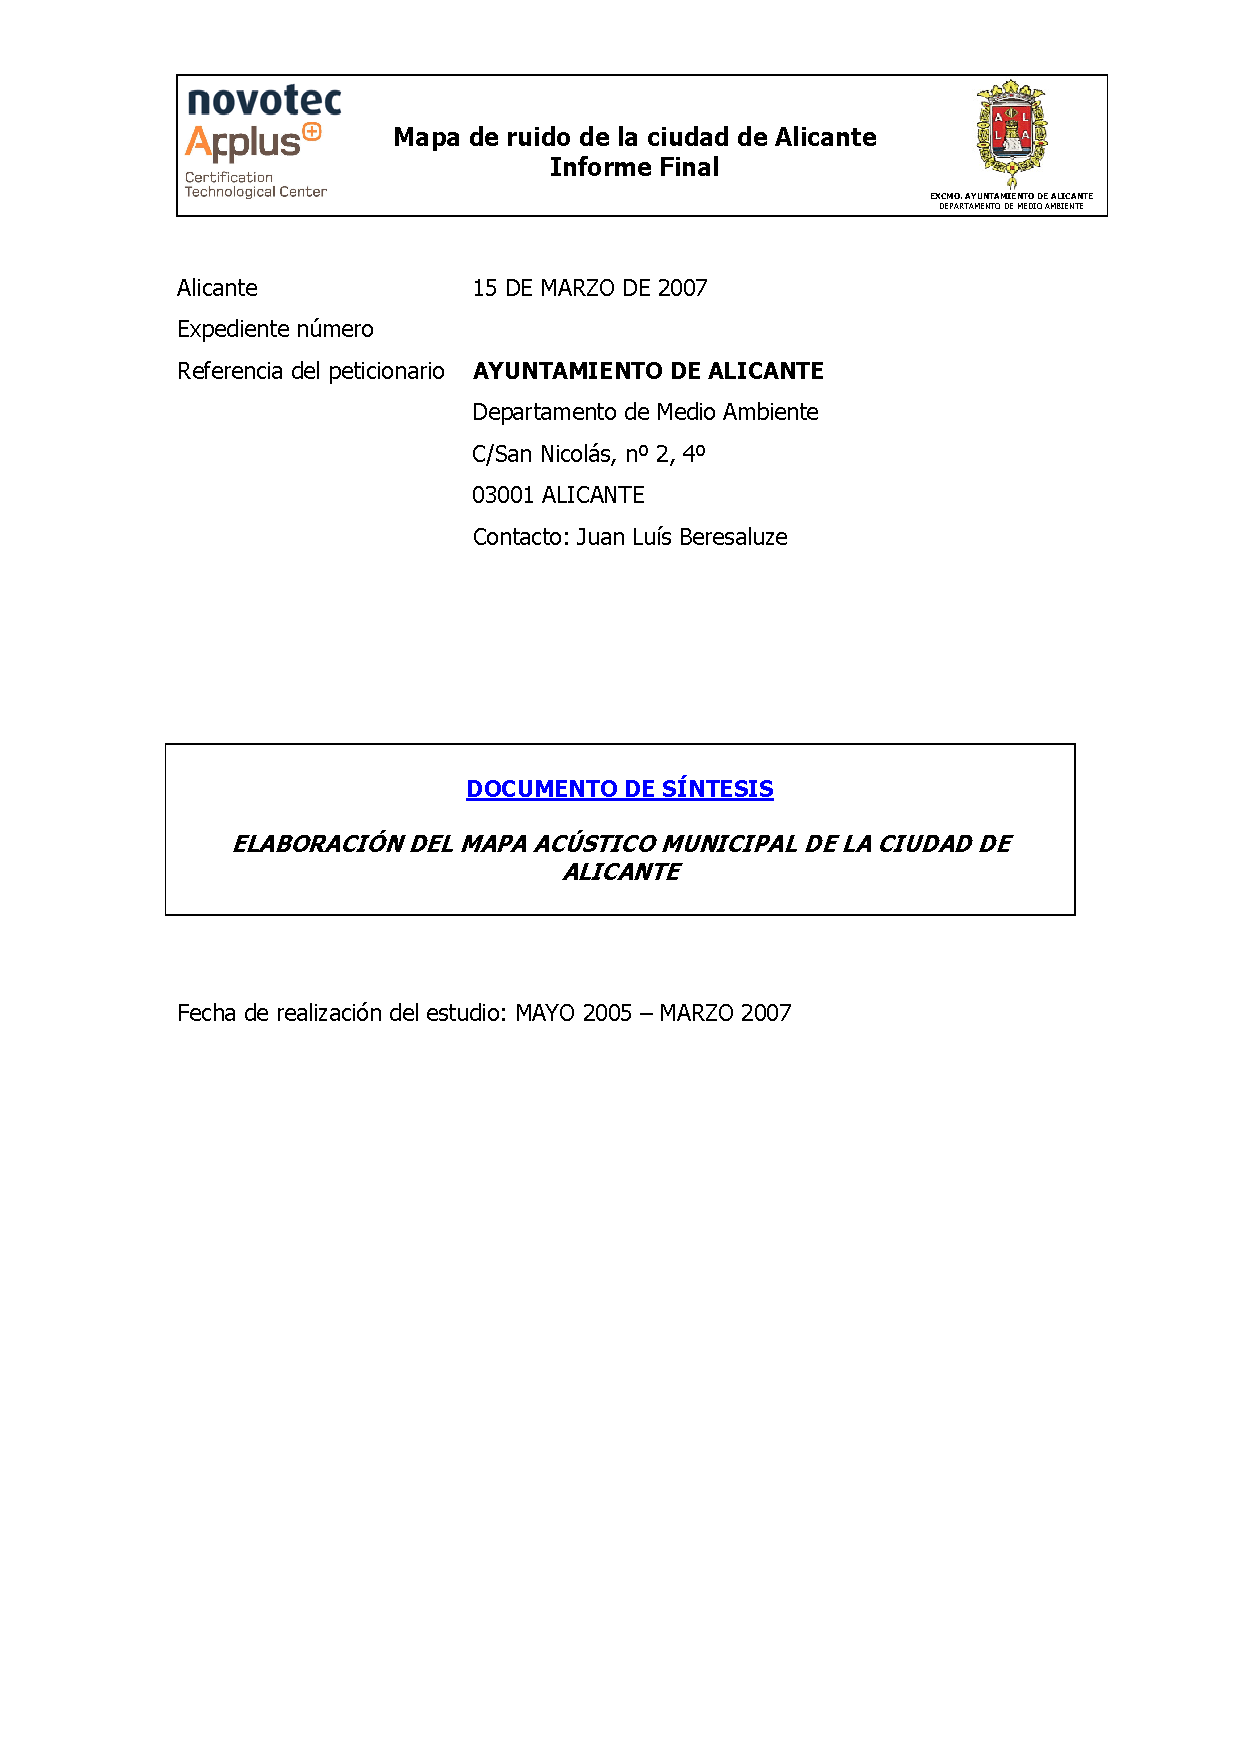
\includepdf[pages={1}]{archivos/ES_a_DF7_Agg_Alicante.pdf}

% Para incluir una página:
% [pages={0}] % Donde '0' es el número de la pagina del PDF que se quiere incluir

% Para incluir varias páginas consecutivas
% [pages={1-4}] % Con estos valores importa de la página 1 a la 4.

% Para incluir varias páginas salteadas
% [pages={1,4,7,10}] % Incluye las páginas 1,4,7 y 10

% Para incluir todo el documento PDF
% [pages=-]

% Si ademas de pages=... se incluye landscape, se importa en horizontal
% [pages{1},landscape]

\end{document}
